\documentclass[showtrims,		% Mostra as marcas de corte em cruz
			   %trimframe,		% Mostra as marcas de corte em linha, para conferência
			   10pt				% 8pt, 9pt, 10pt, 11pt, 12pt, 14pt, 17pt, 20pt 
			   ]{memoir}
\usepackage[brazilian,
			% english,
			% italian,
			% ngerman,
			% french,
			% russian,
			% polutonikogreek
			]{babel}
\usepackage{anyfontsize}			    % para tamanhos de fontes maiores que \Huge 
\usepackage{relsize}					% para aumentar ou diminuir fonte por pontos. Ex. \smaller[1]
\usepackage{fontspec}					% para rodar fontes do sistema
\usepackage[switch]{lineno} 			% para numerar linhas
\usepackage{lipsum}						% para colocar textos lipsum
\usepackage{alltt}						% para colocar espaços duplos. Ex: verso livre
\usepackage{graphicx}					% para colocar imagens
\usepackage{float}						% para flutuar imagens e tabelas 		
\usepackage{lettrine}					% para capsulares
\usepackage{comment}					% para comentar o código em bloco \begin{comment}...
\usepackage{adforn}						% para adornos & glyphs
\usepackage{xcolor}					 	% para texto colorido
\usepackage[babel]{microtype}			% para ajustes finos na mancha
\usepackage{enumerate,enumitem}			% para tipos diferentes de enumeração/formatação ver `edlab-extra.sty`
\usepackage{url}					% para citar sites \url
\usepackage{marginnote}					% para notas laterais
\usepackage{titlesec}					% para produzir os distanciamentos entre pontos no \dotfill

%\usepackage{makeidx} 					% para índice remissivo

\usepackage{edlab-penalties}
\usepackage{edlab-git}
\usepackage{edlab-toc}					% define sumário
\usepackage{edlab-extra}				% define epígrafe, quote
\usepackage[11x18]{edlab-margins}
\usepackage[%semcabeco, 				% para remover cabeço, sobe mancha e mantem estilos
			]{edlab-sections}			% define pagestyle (cabeço, rodapé e seções)
\usepackage[%
			% notasemlinha 			
			% notalinhalonga
			chicagofootnotes			% para notas com número e ponto cf. man. de Chicago
			]{edlab-footnotes}


% Medidas (ver: memoir p.11 fig.2.3)
\parindent=3ex			% Tamanho da indentação
\parskip=0pt			% Entre parágrafos
\marginparsep=1em		% Entre mancha e nota lateral 
\marginparwidth=4em		% Tamanho da caixa de texto da nota laterial

% Fontes
\newfontfamily\formular{Formular}
\newfontfamily\formularlight{Formular Light}
\setmainfont[Ligatures=TeX,Numbers=OldStyle]{Minion Pro}

% Estilos
\makeoddhead{baruch}{}{\scshape\MakeLowercase{\scshape\MakeTextLowercase{}}}{}
\makeevenhead{baruch}{}{\scshape\MakeLowercase{}}{}
\makeevenfoot{baruch}{}{\footnotesize\thepage}{}
\makeoddfoot{baruch}{}{\footnotesize\thepage}{}
\pagestyle{baruch}		
\headstyles{baruch}
\linespread{1.1}

% Testes


\begin{document}


%\book{\textsc{Testis nossis},  Mussum Ipsum}

\part{Amor é fogo que arde sem se ver}

\chapter{É um não querer mais que bem\footnote{Cacilds vidis litro abertis.} querer}

\newcommand{\pacote}[1]{\marginnote{\tiny\alltt{#1}}}


\pacote{edlab-extra}
\begin{epigraphs} 
\qitem{Cogitatio in vero exquirendo maxime versatur. 
		 Appetitus impellit ad agendum.}{\textsc{Marcus
		  Tullius Cicero}}
\end{epigraphs}

\pacote{lettrine.sty}
\lettrine[realheight]{\textcolor{red}{M}}{ussum Ipsum}, cacilds vidis litro abertis. Suco de cevadiss, é um leite
divinis, qui tem lupuliz, a\textcolor{green}{fi}matis, aguis e fermentis. Sapien in monti palavris
qui num significa nadis i pareci latim.  Diuretics paradis num copo é motivis
de denguis. Mauris nec dolor in eros commodo tempor. Aenean aliquam molestie
leo, vitae iaculis nisl. Ligue para \textcolor{green}{9-3129-4563}.


In elementis \url{www.hedra.com.br\~#} mé pra quem é amistosis quis leo. Vehicula non. Ut sed ex eros.
Vivamus sit amet nibh non tellus tristique interdum. Copo furadis é disculpa de
bebadis, arcu quam euismod magna. Todo mundo vê os porris que eu tomo, mas
ninguém vê os tombis que eu levo!

\section{É solitário andar por entre a gente}


Pra lá , depois divoltis porris, paradis. Praesent vel viverra nisi. Mauris
aliquet nunc non turpis scelerisque, eget. Nec orci ornare consequat. Praesent
lacinia ultrices\footnote{Praesent vel viverra nisi. Mauris
aliquet nunc non turpis scelerisque, eget.} consectetur.\footnote{Sed non ipsum.} Sed non ipsum felis. Si u mundo tá muito paradis?
Toma um mé que o mundo vai girarzis!\footnote{\textsc{Mussum}, Ipsum,
\textit{Cacilds vidis litro abertis}.}




Em pé sem cair, deitado sem dormir, sentado sem cochilar e fazendo pose. Quem
num gosta di mé, boa gentis num é. Não sou faixa preta cumpadi, sou preto
inteiris, inteiris. Aenean aliquam molestie leo, vitae iaculis nisl.

\settowidth{\versewidth}{Nay, nay, I leave thee not, thou goest too}
\begin{verse}[\versewidth]
\ldots \\*
His judgement rendered, he dissolved the Thing. \\*
\flagverse{Ingeborg} And your decision? \\*
\flagverse{Fridthjof} \vinphantom{And your decision?}
Have I ought to choose? \\*
Is not mine honour bound by his decree? \\*
And that I will redeem through Angantyr \\*
His paltry gold doth hide in Nastrand’s flood. \\*
Today will I depart. \\*
\flagverse{Ingeborg} \vinphantom{Today will I depart.}
And Ingeborg leave? \\*
\flagverse{Fridthjof} Nay, nay, I leave thee not,
thou goest too. \\*
\flagverse{Ingeborg} Impossible! \\*
\flagverse{Fridthjof} \vinphantom{Impossible!}
O! hear me, ere thou answerest.
\end{verse}

Interagi no mé, cursus quis, vehicula ac nisi. Admodum accumsan disputationi eu
sit. Vide electram sadipscing et per. Detraxit consequat et quo num tendi nada.
Atirei o pau no gatis, per gatis num morreus.

Suco de cevadiss deixa as pessoas mais interessantis. Tá deprimidis, eu conheço
uma cachacis que pode alegrar sua vidis. Praesent malesuada urna nisi, quis
volutpat erat hendrerit non. Nam vulputate dapibus. Quem manda na minha terra
sou euzis!

\subsection{É nunca contentar-se de contente}

Em pé sem cair, deitado sem dormir, sentado sem cochilar e fazendo pose. Quem
num gosta di mé, boa gentis num é. Não sou faixa preta cumpadi, sou preto
inteiris, inteiris. Aenean aliquam molestie leo, vitae iaculis nisl.

Interagi no mé, cursus quis, vehicula ac nisi. Admodum accumsan disputationi eu
sit. Vide electram sadipscing et per. Detraxit consequat et quo num tendi nada.
Atirei o pau no gatis, per gatis num morreus.

\pacote{alltt}
\begin{alltt}\normalfont			%Verso branco
I used to love my garden
But now my love is dead
   For I found a 
   			      		[ bachelor’s button
   In black-eyed 
              	        [ Susan’s bed.
\end{alltt}

Suco de cevadiss deixa as pessoas mais interessantis. Tá deprimidis, eu conheço
uma cachacis que pode alegrar sua vidis. Praesent malesuada urna nisi, quis
volutpat erat hendrerit non. Nam vulputate dapibus. Quem manda na minha terra
sou euzis!

\subsubsection{Posuere libero varius}

Mussum Ipsum, cacilds vidis litro abertis. Posuere libero varius. Nullam a nisl
ut ante blandit hendrerit. Aenean sit amet nisi. Mé faiz elementum girarzis,
nisi eros vermeio. Interessantiss quisso pudia ce receita de bolis, mais bolis
eu num gostis. Diuretics paradis num copo é motivis de denguis.

Per aumento de cachacis, eu reclamis. Todo mundo vê os porris que eu tomo, mas
ninguém vê os tombis que eu levo! Admodum accumsan disputationi eu sit. Vide
electram sadipscing et per. Detraxit consequat et quo num tendi nada.

\chapter{Leite de capivaris, leite de mula manquis sem cabeça}

Leite de capivaris, leite de mula manquis sem cabeça. Suco de cevadiss deixa as
pessoas mais interessantis. Casamentiss faiz malandris se pirulitá. Em pé sem
cair, deitado sem dormir, sentado sem cochilar e fazendo pose.

Praesent vel viverra nisi. Mauris aliquet nunc non turpis scelerisque, eget.
Atirei o pau no gatis, per gatis num morreus. Quem num gosta di mé, boa gentis
num é. Paisis, filhis, espiritis santis.

\settowidth{\versewidth}{É solitário andar por entre a gente;}\label{camoes}
\begin{verse}[\versewidth]
\linenumbers

Amor é fogo que arde sem se ver;\\*
É ferida que dói e não se sente;\\*
É um contentamento descontente;\\*
É dor que desatina sem doer;\\!

É um não querer mais que bem querer;\\*
É solitário andar por entre a gente;\\*
É nunca contentar-se de contente;\\*
É cuidar que se ganha em se perder;\\!

É querer estar preso por vontade;\\*
É servir a quem vence, o vencedor;\\*
É ter com quem nos mata lealdade.\\!

Mas como causar pode seu favor\\*
Nos corações humanos amizade,\\*
Se tão contrário a si é o mesmo Amor?\\!

                 \hfill    \textsc{Luís de Camões}
\end{verse}

\marginnote{\footnotesize \textcolor{green}{Pra lá, depois divoltis porris, paradis. Praesent vel viverra nisi.}}
Delegadis gente finis, bibendum egestas augue arcu ut est. Praesent malesuada
urna nisi, quis volutpat erat hendrerit non. Nam vulputate dapibus. Nullam
volutpat risus nec leo commodo, ut interdum diam laoreet. Sed non consequat
odio. Si num tem leite então bota uma pinga aí cumpadi!

Sapien in monti palavris qui num significa nadis i pareci latim.  Quem num
gosta di mim que vai caçá sua turmis! A ordem dos tratores não altera o pão
duris. Quem manda na minha terra sou euzis!

Não sou faixa preta cumpadi, sou preto inteiris, inteiris. Manduma pindureta
quium dia nois paga. Aenean aliquam molestie leo, vitae iaculis nisl. Si u
mundo tá muito paradis? Toma um mé que o mundo vai girarzis!

Viva Forevis aptent taciti sociosqu ad litora torquent. Cevadis im ampola pa
arma uma pindureta. In elementis mé pra quem é amistosis quis leo. Nec orci
ornare consequat. Praesent lacinia ultrices consectetur. Sed non ipsum felis.
%


%h	Place the float here, i.e., 
% 	   approximately at the same point it 
% 	   occurs in the source text (however, not exactly at the spot)
%t	Position at the top of the page.
%b	Position at the bottom of the page.
%p	Put on a special page for floats only.
%!	Override internal parameters LATEX uses for determining "good" float positions.
%H	Places the float at precisely the location in the LATEX code. 
%	  Requires the float package (\usepackage{float}). This is 
%	  somewhat equivalent to h!, though some errors may 
%	  arise if you have too many consecutive floats with [H].
%   LINK: https://www.overleaf.com/learn/latex/Positioning_of_Figures

\pacote{graphicx}
\begin{figure}[h]
\centering
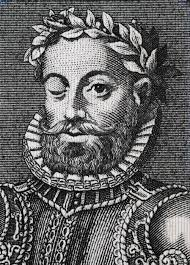
\includegraphics[width=0.5\textwidth]{image}
\caption{Camões Caolhiuos}
\label{fig:camoes}
\end{figure}

Interagi no mé, cursus quis, vehicula ac nisi. Mauris nec dolor in eros commodo
tempor. Aenean aliquam molestie leo, vitae iaculis nisl. Suco de cevadiss, é um
leite divinis, qui tem lupuliz, matis, aguis e fermentis. Copo furadis é
disculpa de bebadis, arcu quam euismod magna.



\paragraph{É cuidar que se ganha em se perder}

Mussum Ipsum, cacilds vidis litro abertis. Mais vale um bebadis conhecidiss,
que um alcoolatra anonimis. Per aumento de cachacis, eu reclamis. Si num tem
leite então bota uma pinga aí cumpadi! Cevadis im ampola pa arma uma pindureta.\footnote{Ver poema na 
		seção \ref{camoes} (p.\,\pageref{camoes}) e também 
		% LINK https://www.overleaf.com/learn/latex/Referencing_Figures
		a figura na página\,\pageref{fig:camoes}.
		\label{notasobrecamoes}}


\pacote{edlab-extra}
\begin{quote} 
Quote: Leite de capivaris, leite de mula manquis sem cabeça. Suco de
cevadiss deixa as pessoas mais interessantis. Casamentiss faiz malandris se
pirulitá. Em pé sem cair, deitado sem dormir, sentado sem cochilar e fazendo
pose.  
\end{quote}

Suco de cevadiss deixa as pessoas mais interessantis. Manduma pindureta quium
dia nois paga. Nec orci ornare consequat. Praesent lacinia ultrices
consectetur. Sed non ipsum felis. Posuere libero varius. Nullam a nisl ut ante
blandit hendrerit. Aenean sit amet nisi.

Vehicula non. Ut sed ex eros. Vivamus sit amet nibh non tellus tristique
interdum. Copo furadis é disculpa de bebadis, arcu quam euismod magna. Mé faiz
elementum girarzis, nisi eros vermeio. Admodum accumsan disputationi eu sit.
Vide electram sadipscing et per.

Casamentiss faiz malandris se pirulitá. Aenean aliquam molestie leo, vitae
iaculis nisl. Paisis, filhis, espiritis santis. Tá deprimidis, eu conheço uma
cachacis que pode alegrar sua vidis.

Suco de cevadiss, é um leite divinis, qui tem lupuliz, matis, aguis e
fermentis. Quem manda na minha terra sou euzis! Quem num gosta di mé, boa
gentis num é. Pra lá , depois divoltis porris, paradis.

A ordem dos tratores não altera o pão duris. Em pé sem cair, deitado sem
dormir, sentado sem cochilar e fazendo pose. Delegadis gente finis, bibendum
egestas augue arcu ut est. Detraxit consequat e
t quo num tendi nada.\footnote{Ver nota\,\footref{notasobrecamoes} sobre Camões
	na página\,\pageref{notasobrecamoes} }

Praesent vel viverra nisi. Mauris aliquet nunc non turpis scelerisque, eget. In
elementis mé pra quem é amistosis quis leo. Não sou faixa preta cumpadi, sou
preto inteiris, inteiris. Interessantiss quisso pudia ce receita de bolis, mais
bolis eu num gostis.

Atirei o pau no gatis, per gatis num morreus. Praesent malesuada urna nisi,
quis volutpat erat hendrerit non. Nam vulputate dapibus. Quem num gosta di mim
que vai caçá sua turmis! Viva Forevis aptent taciti sociosqu ad litora
torquent.

Nullam volutpat risus nec leo commodo, ut interdum diam laoreet. Sed non
consequat odio. Interagi no mé, cursus quis, vehicula ac nisi. Leite de
capivaris, leite de mula manquis sem cabeça. Sapien in monti palavris qui num
significa nadis i pareci latim.

Diuretics paradis num copo é motivis de denguis. Mauris nec dolor in eros
commodo tempor. Aenean aliquam molestie leo, vitae iaculis nisl. Si u mundo tá
muito paradis? Toma um mé que o mundo vai girarzis! Todo mundo vê os porris que
eu tomo, mas ninguém vê os tombis que eu levo!

Interagi no mé, cursus quis, vehicula ac nisi. Viva Forevis aptent taciti
sociosqu ad litora torquent. Quem manda na minha terra sou euzis! Praesent vel
viverra nisi. Mauris aliquet nunc non turpis scelerisque, eget.

Si u mundo tá muito paradis? Toma um mé que o mundo vai girarzis! Atirei o pau
no gatis, per gatis num morreus. Quem num gosta di mé, boa gentis num é. A
ordem dos tratores não altera o pão duris.

Delegadis gente finis, bibendum egestas augue arcu ut est. Mauris nec dolor in
eros commodo tempor. Aenean aliquam molestie leo, vitae iaculis nisl. Mais vale
um bebadis conhecidiss, que um alcoolatra anonimis. Em pé sem cair, deitado sem
dormir, sentado sem cochilar e fazendo pose.

\subparagraph{É querer estar preso por vontade}

Atirei o pau no gatis, per gatis num morreus. Praesent malesuada urna nisi,
quis volutpat erat hendrerit non. Nam vulputate dapibus. Quem num gosta di mim
que vai caçá sua turmis! Viva Forevis aptent taciti sociosqu ad litora
torquent.

Nullam volutpat risus nec leo commodo, ut interdum diam laoreet. Sed non
consequat odio. Interagi no mé, cursus quis, vehicula ac nisi. Leite de
capivaris, leite de mula manquis sem cabeça. Sapien in monti palavris qui num
significa nadis i pareci latim.


Nullam volutpat risus nec leo commodo, ut interdum diam laoreet. Sed non
consequat odio. Interagi no mé, cursus quis, vehicula ac nisi. Leite de
capivaris, leite de mula manquis sem cabeça. Sapien in monti palavris qui num
significa nadis i pareci latim.

Diuretics paradis num copo é motivis de denguis. Mauris nec dolor in eros
commodo tempor. Aenean aliquam molestie leo, vitae iaculis nisl. Si u mundo tá
muito paradis? Toma um mé que o mundo vai girarzis! Todo mundo vê os porris que
eu tomo, mas ninguém vê os tombis que eu levo!

Interagi no mé, cursus quis, vehicula ac nisi. Viva Forevis aptent taciti
sociosqu ad litora torquent. Quem manda na minha terra sou euzis! Praesent vel
viverra nisi. Mauris aliquet nunc non turpis scelerisque, eget.

Si u mundo tá muito paradis? Toma um mé que o mundo vai girarzis! Atirei o pau
no gatis, per gatis num morreus. Quem num gosta di mé, boa gentis num é. A
ordem dos tratores não altera o pão duris.

Delegadis gente finis, bibendum egestas augue arcu ut est. Mauris nec dolor in
eros commodo tempor. Aenean aliquam molestie leo, vitae iaculis nisl. Mais vale
um bebadis conhecidiss, que um alcoolatra anonimis. Em pé sem cair, deitado sem
dormir, sentado sem cochilar e fazendo pose.

\subparagraph{É querer estar preso por vontade}

Atirei o pau no gatis, per gatis num morreus. Praesent malesuada urna nisi,
quis volutpat erat hendrerit non. Nam vulputate dapibus. Quem num gosta di mim
que vai caçá sua turmis! Viva Forevis aptent taciti sociosqu ad litora
torquent.

Nullam volutpat risus nec leo commodo, ut interdum diam laoreet. Sed non
consequat odio. Interagi no mé, cursus quis, vehicula ac nisi. Leite de
capivaris, leite de mula manquis sem cabeça. Sapien in monti palavris qui num
significa nadis i pareci latim.


Nullam volutpat risus nec leo commodo, ut interdum diam laoreet. Sed non
consequat odio. Interagi no mé, cursus quis, vehicula ac nisi. Leite de
capivaris, leite de mula manquis sem cabeça. Sapien in monti palavris qui num
significa nadis i pareci latim.

Diuretics paradis num copo é motivis de denguis. Mauris nec dolor in eros
commodo tempor. Aenean aliquam molestie leo, vitae iaculis nisl. Si u mundo tá
muito paradis? Toma um mé que o mundo vai girarzis! Todo mundo vê os porris que
eu tomo, mas ninguém vê os tombis que eu levo!

Interagi no mé, cursus quis, vehicula ac nisi. Viva Forevis aptent taciti
sociosqu ad litora torquent. Quem manda na minha terra sou euzis! Praesent vel
viverra nisi. Mauris aliquet nunc non turpis scelerisque, eget.

Si u mundo tá muito paradis? Toma um mé que o mundo vai girarzis! Atirei o pau
no gatis, per gatis num morreus. Quem num gosta di mé, boa gentis num é. A
ordem dos tratores não altera o pão duris.

Delegadis gente finis, bibendum egestas augue arcu ut est. Mauris nec dolor in
eros commodo tempor. Aenean aliquam molestie leo, vitae iaculis nisl. Mais vale
um bebadis conhecidiss, que um alcoolatra anonimis. Em pé sem cair, deitado sem
dormir, sentado sem cochilar e fazendo pose.

\subparagraph{É querer estar preso por vontade}

Atirei o pau no gatis, per gatis num morreus. Praesent malesuada urna nisi,
quis volutpat erat hendrerit non. Nam vulputate dapibus. Quem num gosta di mim
que vai caçá sua turmis! Viva Forevis aptent taciti sociosqu ad litora
torquent.

Nullam volutpat risus nec leo commodo, ut interdum diam laoreet. Sed non
consequat odio. Interagi no mé, cursus quis, vehicula ac nisi. Leite de
capivaris, leite de mula manquis sem cabeça. Sapien in monti palavris qui num
significa nadis i pareci latim.


Nullam volutpat risus nec leo commodo, ut interdum diam laoreet. Sed non
consequat odio. Interagi no mé, cursus quis, vehicula ac nisi. Leite de
capivaris, leite de mula manquis sem cabeça. Sapien in monti palavris qui num
significa nadis i pareci latim.

Diuretics paradis num copo é motivis de denguis. Mauris nec dolor in eros
commodo tempor. Aenean aliquam molestie leo, vitae iaculis nisl. Si u mundo tá
muito paradis? Toma um mé que o mundo vai girarzis! Todo mundo vê os porris que
eu tomo, mas ninguém vê os tombis que eu levo!

Interagi no mé, cursus quis, vehicula ac nisi. Viva Forevis aptent taciti
sociosqu ad litora torquent. Quem manda na minha terra sou euzis! Praesent vel
viverra nisi. Mauris aliquet nunc non turpis scelerisque, eget.

Si u mundo tá muito paradis? Toma um mé que o mundo vai girarzis! Atirei o pau
no gatis, per gatis num morreus. Quem num gosta di mé, boa gentis num é. A
ordem dos tratores não altera o pão duris.

Delegadis gente finis, bibendum egestas augue arcu ut est. Mauris nec dolor in
eros commodo tempor. Aenean aliquam molestie leo, vitae iaculis nisl. Mais vale
um bebadis conhecidiss, que um alcoolatra anonimis. Em pé sem cair, deitado sem
dormir, sentado sem cochilar e fazendo pose.

\subparagraph{É querer estar preso por vontade}

Atirei o pau no gatis, per gatis num morreus. Praesent malesuada urna nisi,
quis volutpat erat hendrerit non. Nam vulputate dapibus. Quem num gosta di mim
que vai caçá sua turmis! Viva Forevis aptent taciti sociosqu ad litora
torquent.

Nullam volutpat risus nec leo commodo, ut interdum diam laoreet. Sed non
consequat odio. Interagi no mé, cursus quis, vehicula ac nisi. Leite de
capivaris, leite de mula manquis sem cabeça. Sapien in monti palavris qui num
significa nadis i pareci latim.
  		% Teste da classe
% Este documento tem a ver com as partes do LIVRO. 

% Tamanhos
% \tiny
% \scriptsize
% \footnotesize
% \small 
% \normalsize
% \large 
% \Large 
% \LARGE 
% \huge
% \Huge

% Posicionamento
% \centering 
% \raggedright
% \raggedleft
% \vfill 
% \hfill 
% \vspace{Xcm}   % Colocar * caso esteja no começo de uma página. Ex: \vspace*{...}
% \hspace{Xcm}

% Estilo de página
% \thispagestyle{<<nosso>>}
% \thispagestyle{empty}
% \thispagestyle{plain}  (só número, sem cabeço)
% https://www.overleaf.com/learn/latex/Headers_and_footers

% Compilador que permite usar fonte de sistema: xelatex, lualatex
% Compilador que não permite usar fonte de sistema: latex, pdflatex

% Definindo fontes
% \setmainfont{Times New Roman}  % Todo o texto
% \newfontfamily\avenir{Avenir}  % Contexto

% \begin{textblock*}{2.625in}(0pt,0pt)%
% \vspace*{-2cm}
% \hspace*{-6.3cm}
% 
\includegraphics[scale=0.7]{./FRONTE/FRONTE.pdf}
% \end{textblock*}   

\thispagestyle{empty}

\begingroup

\mbox{}
\centering
\vfill

\includegraphics[scale=0.11]{./FRONTE/FRONTE.pdf}
\vfill
\mbox{}

\endgroup
\pagebreak       % [Frontistício]
%\newcommand{\linhalayout}[2]{{\tiny\textbf{#1}\quad#2\par}}
\newcommand{\linha}[2]{\ifdef{#2}{\linhalayout{#1}{#2}}{}}

\begingroup\tiny
\parindent=0cm
\thispagestyle{empty}

\textbf{copyright}\quad {Chaim Novodvorsky}\\
\textbf{edição brasileira©}\quad			 {Hedra \the\year}\\
\textbf{tradução©}\quad			 			 {Léa Baran}\\
\textbf{organização©}\quad			 		 {Lilian Starobinas}\\
\textbf{prefácio©}\quad			 			 {Roney Cytrynowicz}\\
%\textbf{ilustração©}\quad			 		 {copyrightilustracao}\medskip

%\textbf{título original}\quad			 	 {titulooriginal}\\
%\textbf{edição consultada}\quad			 	 {edicaoconsultada}\\
\textbf{primeira edição}\quad			 	 {}\\
%\textbf{agradecimentos}\quad			 	 {agradecimentos}\\
%\textbf{indicação}\quad			 			 {indicacao}\medskip

\textbf{edição}\quad			 			 {Suzana Salama}\\
%\textbf{coedição}\quad			 			 {coedicao}\\
\textbf{assistência editorial}\quad			 {Paulo Henrique Pompermaier}\\
%\textbf{revisão}\quad			 			 {revisao}\\
%\textbf{preparação}\quad			 		 {preparacao}\\
%\textbf{iconografia}\quad			 		 {iconografia}\\
\textbf{capa}\quad			 				 {Lucas Kroëff}\\
%\textbf{imagem da capa}\quad			 	 {imagemcapa}\medskip

\textbf{ISBN}\quad			 				 {ISBN}\smallskip

%\hspace{-5pt}\begin{tabular}{ll}
%\textbf{conselho editorial} & Adriano Scatolin,  \\
%							& Antonio Valverde,  \\
%							& Caio Gagliardi,    \\
%							& Jorge Sallum,      \\
%							& Ricardo Valle,     \\
%							& Tales Ab'Saber,    \\
%							& Tâmis Parron      
%\end{tabular}
 

\vfill

\textit{Grafia atualizada segundo o Acordo Ortográfico da Língua\\
Portuguesa de 1990, em vigor no Brasil desde 2009.}\\

\textit{Direitos reservados em língua\\ 
portuguesa somente para o Brasil}\\\medskip

\textsc{ayllon editora ltda.}\\
R.~Fradique Coutinho, 1139\\
05416--011 São Paulo \textsc{sp} Brasil\\
Telefone/Fax +55 11 3097 8304\\\smallskip
editora@hedra.com.br\\
www.hedra.com.br\\
\bigskip
Foi feito o depósito legal.

\endgroup
\pagebreak     % [Créditos]
% Tamanhos
% \tiny
% \scriptsize
% \footnotesize
% \small 
% \normalsize
% \large 
% \Large 
% \LARGE 
% \huge
% \Huge

% Posicionamento
% \centering 
% \raggedright
% \raggedleft
% \vfill 
% \hfill 
% \vspace{Xcm}   % Colocar * caso esteja no começo de uma página. Ex: \vspace*{...}
% \hspace{Xcm}

% Estilo de página
% \thispagestyle{<<nosso>>}
% \thispagestyle{empty}
% \thispagestyle{plain}  (só número, sem cabeço)
% https://www.overleaf.com/learn/latex/Headers_and_footers

% Compilador que permite usar fonte de sistema: xelatex, lualatex
% Compilador que não permite usar fonte de sistema: latex, pdflatex

% Definindo fontes
% \setmainfont{Times New Roman}  % Todo o texto
% \newfontfamily\avenir{Avenir}  % Contexto

\begingroup\thispagestyle{empty}\vspace*{.05\textheight} 

              \formular
              \huge
              \noindent
              \textsc{Em busca de meus irmãos\\na América}
  					  \medskip
                      
  					  \large
              \textit{}
              \normalsize 
              \vspace{2em}

              \Large
              \noindent
              \textbf{Chaim Novodvorsky}
              \bigskip

              \small
              \noindent
              Lilian Starobinas (\textit{organização})\\
              Léa Baran (\textit{tradução})
              \vspace{3em}

              \noindent
   					  1ª Edição
                      

              \vfill
              \noindent
              %\newfontfamily\timesnewroman{Times New Roman}
              %{\fontsize{30}{40}\selectfont \timesnewroman hedra}
              %\smallskip
              
\includegraphics[width=0.3\textwidth]{logo}
              \break{} São Paulo\quad\the\year
              %São Paulo \the\year
\endgroup
\pagebreak
	       % [folha de rosto]
% nothing			is level -3
% \book				is level -2
% \part				is level -1
% \chapter 			is level 0
% \section 			is level 1
% \subsection 		is level 2
% \subsubsection 	is level 3
% \paragraph 		is level 4
% \subparagraph 	is level 5
\setcounter{secnumdepth}{-2}
\setcounter{tocdepth}{0}

% \renewcommand{\contentsname}{Índex} 	% Trocar nome do sumário para 'Índex'
%\ifodd\thepage\relax\else\blankpage\fi 	% Verifica se página é par e coloca página branca
%\tableofcontents*

\pagebreak
\begingroup \footnotesize \parindent0pt \parskip 5pt \thispagestyle{empty} \vspace*{-0.5\textheight}\mbox{} \vfill
\baselineskip=.92\baselineskip
\textbf{Chaim Novodvorsky} (Knishin, Polônia, 1902--São Paulo, 1983) \textls[-10]{deixou sua família em um pequeno vilarejo polonês aos 19 anos com o objetivo de imigrar para os Estados Unidos: parte dos irmãos já estava na América e ele fugia do serviço militar, um dos mais frequentes motivos de emigração da Europa Oriental e do Império Russo desde o século \textsc{xix}. Diante da recusa de visto, lançou-se de toda forma rumo ao outro lado do mundo e trabalhou nas mais diversas profissões --- como padeiro, mascate, leitor de realejo, comerciante, lojista, importador, fabricante. Além disso, construiu uma história de vida que perpassa temas importantes da história judaica e sul-americana, como a passagem por Moisés Ville, colônia agrícola fundada pela Jewish Colonization Association na Argentina; a atuação no teatro iídiche; a participação ativa nas instituições comunitárias; e a doação de aviões à recém-criada Força Aérea Brasileira durante a \textsc{ii} Guerra Mundial.}

\textbf{Em busca de meus irmãos na América} é um relato pessoal singular e ao mesmo tempo emblemático dos percursos da imigração judaica entre os anos 1920 e 1960. Novodvorsky, que imigrou primeiro para a Argentina, depois para o Uruguai e, finalmente, para o Brasil, construiu esse roteiro longo em função de um objetivo final e aspirado, que era o deslocamento para os Estados Unidos. Suas memórias também revelam fatores estruturais que caracterizaram o estabelecimento dos judeus no Brasil, como as barreiras impostas à imigração em países como Estados Unidos e Canadá durante a década de 1920, que fizeram do país um horizonte possível e desejável.

\pagebreak

\textbf{Lilian Starobinas} \textls[-10]{é neta de Chaim Novodvorsky. Historiadora e doutora em educação pela \textsc{usp}, é professora de história na Escola Vera Cruz, onde leciona também no curso de pedagogia. Junto a vários autores, publicou \textit{Vanguarda pedagógica: o legado do Ginásio Israelita Brasileiro Scholem Aleichem}, além de diversos artigos sobre a presença judaica no Brasil e teatro ídiche. É membro da coordenação dos coletivos Círculo de Reflexão sobre Judaísmo Contemporâneo e Trupe Ídiche, ambos na Casa do Povo.}\looseness=-1

\textbf{Léa Baran} (Rechitsa, Bielorrussia, 1927--São Paulo, 2016) foi professora, além de tradutora do iídiche e do russo.

\textbf{Roney Cytrynowicz} é historiador, doutor em história pela \textsc{usp}, diretor da Narrativa Um e autor, entre outros, de \textit{Guerra sem guerra: a mobilização e o cotidiano em São Paulo durante a Segunda Guerra Mundial} (2000) e \textit{Memória da barbárie: a história do genocídio dos judeus} (1990), ambos publicados pela Edusp. Foi diretor de acervo do Arquivo Histórico Judaico Brasileiro.\looseness=-1





\endgroup

\pagebreak\thispagestyle{empty}\movetooddpage
{\begingroup\mbox{}\pagestyle{empty}
\pagestyle{empty} 
% \renewcommand{\contentsname}{Índex} 	% Trocar nome do sumário para 'Índex'
%\ifodd\thepage\relax\else\blankpage\fi 	% Verifica se página é par e coloca página branca
\addtocontents{toc}{\protect\thispagestyle{empty}}
\tableofcontents*\clearpage\endgroup}

\newcommand{\subtitulo}[1]{\NoCaseChange{\textnormal{\break\Large\itshape#1}}}
\chapter*{Apresentação\smallskip\subtitulo{Um \emph{road movie} em forma\\de narrativa}}
\markboth{Apresentação}{Lilian Starobinas}
\addcontentsline{toc}{chapter}{Apresentação, \textit{por Lilian Starobinas}}


\begin{flushright}
\textsc{lilian starobinas}
\end{flushright}\medskip

\noindent{}Das páginas manuscritas em iídiche, agora amareladas pelo tempo, numa
caligrafia miúda e regular, provém essas histórias que compõem a
autobiografia de meu avô. Foram registradas por ele no ano de 1964, num
caderno que se tomou um tesouro familiar. Seu Jaime, como o chamávamos,
viveu ainda mais duas décadas, mas nunca se preocupou em escrever suas
memórias em português. Contá-las oralmente sim, ele que era um grande
contador de histórias, bom de papo, comunicativo. Assim, muitas das
passagens que publicamos agora, traduzidas, fazem parte do repertório que
escutávamos o vovô contar, e que foram construindo nossa memória sobre
as origens da família.

\section{sobre a tradução}

Foi a filha mais nova, Cecília, minha mãe, quem tomou para si o desafio
de publicar o livro, e assim trazer a público as narrativas sobre a
trajetória de imigração e estabelecimento no Brasil de seu pai. Mais que
uma homenagem, ela teve consciência da singularidade desse material e da
contribuição que ele traz para a história dos processos de imigração.

Ao longo dos anos, ela empenhou-se para conseguir quem traduzisse.
Inicialmente, investiu num processo artesanal, com a ajuda da sogra,
minha avó Rosa Starobinas, que lia em voz alta o texto e traduzia os
trechos na sequência, enquanto minha mãe registrava sua versão no
gravador com fita cassete. Sem sucesso em fazer a tradução por completo,
decidiu procurar quem fizesse profissionalmente, e assim chegou em Léa
Baran. Entre a tradução e a publicação passaram-se ainda alguns anos.
Finalmente conseguimos compartilhar com mais leitores essas saborosas
histórias de Chaim Novodvorsky.

\section{o contexto histórico}

A Polônia é seu lugar de origem. Viviam ali, estima-se, mais de
3 milhões de judeus antes da Segunda Guerra Mundial. A comunidade
judaica de Knishin, o \textit{shtetl}\footnote{Do iídiche, ``cidadezinha''. O termo se aplica a povoações ou bairros de cidades com população predominantemente judaica.} onde nasceu o autor deste livro, contava com cerca de 3.500 membros em 1900, e 1.235 em 1921. Perto dali ficava Bialistok, uma comunidade muito maior, que passava dos 40 mil habitantes judeus na
década de 1920. 

A intensificação do processo de emigração se deu a partir das primeiras décadas do século \textsc{xx}, diante das duras condições econômicas, dos riscos físicos representados pelos
\textit{pogroms},\footnote{Termo usado para descrever um ataque violento massivo, com destruição de casas, negócios, centros religiosos. Atribuído à perseguição deliberada de um grupo étnico ou religioso, aprovado ou tolerado pelas autoridades locais.} das destruições e horrores frutos da Primeira Guerra Mundial,
das incertezas provocadas pela eclosão da Revolução Russa e das
instabilidades políticas por toda a Europa. Tornou-se frequente, dentre os
judeus da Europa Oriental, o desejo de estabelecerem-se nos Estados
Unidos, país visto como terra das oportunidades e da liberdade de
religião, dando origem à expressão \textit{fazer a América}. Paralelamente estruturava-se o movimento sionista, que estimulava a imigração para a Palestina. O desejo de construir um lar nacional judaico passou a ser defendido como necessário para a uma existência autônoma e livre das perseguições vivenciadas por judeus em diferentes países da Europa ao longo da história. 

Entre 1880 e 1914, partiram cerca de dois milhões de judeus
asquenazitas, provenientes da Europa Oriental, de regiões que formavam o
Pale (zonas de residências permitidas ao judeus). Trata-se de uma área
situada em terras pertencentes ao Império Russo, ao Império
Austro-Húngaro, à Prússia e à Romênia. Chegaram aos Estados Unidos.
Falantes do iídiche, representaram notória influência na cultura local,
na produção literária e nos campos da música, do teatro, do cinema, das
artes em geral. A partir de 1921, os Estados Unidos estabeleceram uma
lei de emergência limitando a imigração, provocada pelo expressivo
aumento de imigrantes após o final da Primeira Guerra Mundial, momento
em que se instaurou uma profunda recessão econômica na Europa.\looseness=-1

A imigração para a América do Sul colocou-se como uma alternativa às
restrições norte-americanas. Desde o final do século \textsc{xix}, ampliou-se a
adoção da Argentina como porto de destino, e estima-se que, até 1920, o
número de imigrantes judeus tenha chegado a cerca de 150 mil. Parte
desse contingente estabeleceu-se em colônias agrícolas, criadas pela
Jewish Colonization Association, uma iniciativa filantrópica voltadas à
absorção de imigrantes e sua inserção econômica nos países de destino.
Uruguai, Brasil, Paraguai e Chile, entre outros países da região,
receberam imigrantes judeus, e viveram o processo de formação de
comunidades locais, com instituições voltadas ao atendimento das
necessidades desses imigrantes e espaços para formação educacional e
religiosa, produção cultural e sociabilidade, sociedades voltadas aos
cuidados de saúde e de sepultamento.

A narrativa de \textit{Em busca de meus irmãos na América} nos permite 
saber mais sobre aspectos dessas redes
de solidariedade formada por imigrantes com referenciais culturais
similares, dando a conhecer não só os sucessos dessas relações, mas
também suas tensões. Encontramos nela as disputas por trabalho, os
estelionatários vendendo ilusões, episódio de discriminação entre os
próprios imigrantes, compondo uma história pouco preocupada com
romantizar a trajetória pessoal. Também se fazem presentes 
os acolhimentos e a ajuda mútua, a valorização dos esforços e do
caráter, as oportunidades de integração e de melhoria das condições de
vida. Chegando na Argentina, no começo dos anos 1920, Chaim deposita
seus esforços no projeto de ir ao encontro dos irmãos, que imigraram
para os Estados Unidos. E assim vai construindo seu percurso em direção
ao norte, escolhendo pontos intermediários nessa rota até seu destino
ideal. Esse traçado dá à narrativa um clima de \textit{road-movie}, pelos
encontros inusitados, a precariedade das situações, a diversidade de
cultura e costumes com as quais ele se depara, a insistência em cumprir
seu destino autoproclamado.\looseness=-1

No coração dessa jornada se encontra o Brasil, e parte importante dessas
memórias está ligada a este país. Mais de quatro milhões de imigrantes
somaram-se à população brasileira, de 1872 até 1940, e entre eles
estima-se a chegada de 60 mil judeus. A imigração judaica deu origem a
comunidades no Rio de Janeiro e em São Paulo, mas também em Porto Alegre,
Curitiba, Belo Horizonte, Salvador, Recife, Belém, além de núcleos
menores fora das capitais. Intensificou-se nos anos 1920, período em que a
politica imigratória dos Estados Unidos sofreu um revés.\looseness=-1

Quase cem anos depois da chegada de Chaim Novodvorsky,
estima-se que há 120 mil judeus no país. Instituições de apoio,
escolas, clubes, sinagogas, escritores e círculos de leitura, teatros,
corais, conjuntos musicais, restaurantes, uma ampla e rica diversidade
de produções e convivências permeiam a vida judaica hoje no Brasil.
Entre associações e disputas, em meio a tempos mais brandos ou mais
difíceis no que diz respeito à vida política e econômica, seguem
compondo comunidades que exercitam o acolhimento ao estrangeiro, valor
de enorme importância na tradição judaica.


\chapter{Capítulo \textsc{ii}}

Desembarquei em Buenos Aires, quase não tinha dinheiro, não sabia falar
o idioma. Soube que existia a Casa dos Imigrantes, pertencente ao
governo.

Tinha trazido comigo o endereço de uma senhora cujos pais eram nossos
vizinhos em Knishin. Eu não a conhecia, ela já morava há muitos anos
ali. Tomei o bonde e fui procurá-la tendo o endereço que seus pais
tinham me dado. E encontrei!

``Sou filho de Elie Novodvorsky, e neto de Chaim Shneguevitch'', me
apresentei, logo ela entendeu quem eu era.

O casal tinha sete filhos, três meninas e quatro meninos, o filho mais
velho era casado. Todos eles moravam numa sala, quer dizer, num quarto
grande, que era divido com um biombo. Na frente havia uma loja, onde
eles vendiam cigarros e ao lado um pequeno espaço que era alugado por um
barbeiro. À noite, eles colocavam camas para o casal e também para as
crianças, separadas com o biombo. Logo vi que não teria lugar ali para
mim.

Voltei então para a Casa dos Imigrantes, pois tinha permissão de dormir
lá durante trinta dias.

Embora eu não tivesse nenhuma profissão, comecei a procurar qualquer
serviço para sobreviver. Comprei um jornal ídiche e vi um anúncio:
``Precisa-se um padeiro''. Pensei ``deve ser um trabalho bom'', achei
que não seria pesado. Imagine, só misturar a farinha com água. Eu
lembrei que sempre observava o nosso vizinho fazendo o pão, ele era um
bom padeiro.

Dirigi-me ao endereço indicado no anúncio e me apresentei como padeiro.
O dono da padaria chamava-se Chaikel e o estabelecimento ficava na rua
Junin, entre as avenidas Corrientes e Lavalle. Ele pediu que voltasse ao
anoitecer para fazer o teste. Era sexta-feira, quando cheguei lá me
perguntou se eu sabia sovar a massa, eu respondi que na minha cidade não
tínhamos este hábito de sovar, e ele logo viu que eu não era padeiro.
Mesmo assim ele me deixou ficar, para não andar de noite pelas ruas que
eu ainda não conhecia. Ajudei a lavar as assadeiras e formas de pão e de
pão doce. Ele me ofereceu chá--mate, tão doce e denso que até grudou nos
meus lábios, eu nunca tinha provado. Eu aceitei e não disse nada, porque
que era um \textit{griner}\footnote{Imigrante recém chegado.} e não queria
que rissem de mim.

Trabalhei a noite inteira, dormi um pouco e de madrugada ele me acordou
e disse: ``Meu jovem você não é padeiro'', ao que eu retruquei ``preciso
trabalhar, porque não tenho ninguém aqui, estou na Casa do Imigrante e
tenho que ganhar o meu sustento''. Ele então disse que eu poderia ficar
e trabalhar como peão, eu nem sabia o que era isso, mas aceitei. Depois
fiquei sabendo que ``peão'' é uma pessoa que faz todo tipo de serviço
que precisa ser feito na padaria. Na minha terra isso era chamado de
carregador.

Sábado de manhã chegou um carregamento de farinha. Tive que descarregar
rápido, só que em vez de colocar nas costas, como na minha terra,
jogaram em cima do ombro, com tanta força que quase caí. Nem podia
reclamar, pois ainda não sabia falar espanhol. Quando terminei com os
sacos de farinha, chegou um vagão de sal, comecei novamente a
descarregar. O sal estava molhado e pesava muito. Foi colocado em
grandes cestas lotadas, e eu novamente não podia dizer nada, pois não
sabia como falar isso em espanhol. Terminei este trabalho ao meio dia.

Às 14 horas comecei a entregar o pão preto nas pequenas mercearias, até
as 17 horas. Continuei trabalhando nesta padaria com direito a
alimentação e a dormir no emprego. Levantava de madrugada, às quatro
horas da manhã distribuía o pão para as pessoas que entregavam no
veículo para os fregueses que moravam mais longe, para os
estabelecimentos onde o pão era vendido. Assim era o meu trabalho todo
dia, além de entregar o açúcar para os padeiros que assavam o pão doce,
bolos, etc.

Neste tempo apareceu um ladrão que roubava o açúcar. Eu reparei que os
sacos estavam diminuindo de quantidade, quando eu deixava de um dia para
o outro. Comecei a observar as pessoas que tinham as chaves e acesso à
padaria e podiam entrar de madrugada. Os sacos ficavam bem próximos da
entrada, em um compartimento. Um rapaz chegava mais cedo do que os
outros, e eu já desconfiava dele. Acordei mais cedo e fiquei esperando
escondido, então vi que ele já estava ali fazia tempo quando os outros
da turma dos padeiros chegaram. Então todos juntos tomaram mate, ele não
me viu, sai e procurei dentro do veículo dele. Debaixo do assento
estavam pequenos sacos de açúcar. Despertei o dono e o levei até o carro
para mostrar que ele estava sendo roubado.

Trabalhei na padaria dois meses, tinha folga nos domingos apenas quatro
horas, fazia o serviço que anteriormente duas pessoas realizavam. Estava
muito cansado, mas a esposa do meu patrão ainda achou que era pouco e
tirou estas quatro horas de folga, me obrigando a limpar a loja. Ela
queria me transformar em um escravo.

Aos domingos eu aproveitava esse curto espaço de tempo para me encontrar
com meus ``irmãos de navio'' em um restaurante. Contei o que estava
acontecendo e resolvemos que eu não voltaria para padaria naquele
momento, só à noite. Cheguei bem tarde e não levantei de madrugada para
trabalhar. O patrão começou a me acordar, eu dei uma desculpa e ele
achou que eu estava doente e não assumi o trabalho que costumava fazer
de manhã. Mais tarde pedi a conta e disse que não iria mais trabalhar na
padaria. Ele me pagou o que quis, 30 pesos no mês. Antes duas pessoas
trabalhavam fazendo meu serviço e recebiam 60 pesos cada um. Foi uma
exploração que cometeram porque eu era ``gringo'' e não tinha ninguém
para me defender. Então fui embora.

\chapter{Capítulo \textsc{iii}}

Enfrentei um novo problema: encontrar um quarto para poder dormir. Sem
profissão, não conseguiria pagar sozinho um quarto e o que recebi do meu
antigo patrão precisava guardar para minha alimentação.

Na Corrientes, encontrei os meus ``irmãos de navio''\footnote{Irmãos de navio, \textit{shif brider}, é a expressão utilizada para identificar imigrantes recém-chegados.} e contei o que estava acontecendo comigo.
Eles então me disseram que eu podia dormir com eles, mas que teria de
entrar bem tarde da noite, escondido, para o senhorio não perceber a
minha presença. Aceitei. Toda noite um deles me aguardava perto da porta
e fazia sinal quando eu podia entrar, mas não havia espaço, as camas
eram de solteiro, e eles dormiam dois em cada cama. Só sobrava um lugar
no chão, onde passei a dormir.

Acordava bem cedo e os donos da pensão nunca ficaram sabendo que estava
dormindo com os meus amigos. Para comer, ia na cantina que foi
organizada para os novos imigrantes que ainda não tinham conseguido
trabalho. A alimentação era barata, porque não poderia pagar o preço de
80 centavos em outros restaurantes e nessa cantina custava só 30
centavos. Quem não podia não pagava nada, comia de graça.

A coletividade judaica tinha boas pessoas que colaboravam com os
\textit{griner}, não os deixando passar fome, demonstrando solidariedade e
organizando cozinhas e cantinas populares. Além das refeições, era mais
fácil também conseguir um emprego nesses lugares, porque os empresários
vinham procurar mão de obra não especializada, como era o meu caso.

Na sexta-feira à noite, apareceu um senhor e se aproximou da mesa onde
eu estava sentado comendo e perguntou:

``Quem de vocês está precisando de trabalho''?

Eu rapidamente dei um pulo e gritei:

``Eu necessito muito trabalhar'', embora não soubesse sobre o que era o
trabalho.

O senhor disse:

``Termine a sua refeição, eu vou esperar''.

``Já acabei'', respondi, pois não conseguia comer de jeito algum, fiquei
com receio que ele falasse com outra pessoa. ``Estou satisfeito podemos
ir''!

Tomamos o bonde e fomos juntos até a casa dele, eu nem perguntei qual
era o serviço que ia fazer, o importante era ter um trabalho. Quando
chegamos lá ele me apresentou para a família, e me explicou sobre o
trabalho que iria fazer, que o filho dele iria me ensinar.

Meu patrão tinha uma pequena fábrica de cigarros especiais, que
entregava de encomenda para uma clientela selecionada: médicos,
advogados, pessoas ricas. Além de ajudar os trabalhadores na fabricação
dos cigarros, eu deveria levar e entregar a domicilio as encomendas e
limpar a loja que ficava na frente da casa.

Fiquei trabalhando lá, com direito as refeições e moradia, e ainda
recebia gorjetas dos fregueses satisfeitos quando fazia entregas. O meu
patrão e a família gostavam de mim porque eu era leal, de toda
confiança, e eles me levavam para todas as festas onde eram convidados.

Trabalhei com eles quatro meses. Todos os domingos eu ia a Rua
Corrientes, a um restaurante cujo dono se chamava Charles, lá eu
encontrava os meus amigos, os ``irmão de navio'', e ouvia notícias do
que estava acontecendo no mundo.

Fiquei então sabendo sobre um trabalho no interior da Argentina, na
época da colheita. Ceifando se ganhava muito bem, embora fosse um
trabalho pesado, desde o amanhecer até o pôr do sol. A vantagem era que
não se gastava nada do dinheiro, guardava-se tudo, pois não tinha o que
comprar. Trabalhando alguns meses, você ficava com uma boa quantia.

Eu achei este trabalho excelente, e não conseguia tirar a ideia da minha
cabeça. Resolvi viajar imediatamente.

Quando cheguei em casa à noite, contei aos meus patrões a minha
resolução:

``Tenho a oportunidade de ganhar um bom dinheiro, porque eu preciso
partir para América para me reunir aos meus irmãos''.

Meu patrão, sua mulher e os filhos começaram a me advertir que este
trabalho era muito pesado, e as minhas mãos não estavam preparadas, eram
muito delicadas, que eu não ia suportar, poderia até adoecer. Mas eu não
quis ouvir nada, nem saber dos conselhos, pensava só em ganhar bastante
dinheiro e ir me encontrar com meus irmãos na América. Eu já sabia que
com dinheiro conseguiria obter um passaporte argentino, como se eu já
vivesse ali há cinco anos, e desse modo não teria nenhum impedimento
para viajar para América. Então me preparei para ir ao interior da
Argentina, para trabalhar na colheita.

Já estava terminando o ano 1922.

\chapter{Capítulo \textsc{iv}}

Fui até a estação de trem para embarcar e viajar até
Mosesville\footnote{Mosesville é uma colônia agrícola fundada na província de
  Santa Fé, na Argentina, em 1889, com objetivo de proporcionar aos
  imigrantes judeus a oportunidade de se tornarem agricultores. Foi uma
  das colônias da Jewish Colonization Association, instituição
  filantrópica fomentada pelo Barão Hirsch.}, uma cidade pequena onde
havia muitos judeus. Cheguei pela manhã, encontrei alguns coches
atrelados aguardando passageiros, pois naquele tempo não havia
automóveis para transporte, nem ônibus.

O cocheiro me perguntou para onde estava indo, respondi que iria
trabalhar na colheita. Ele me olhou e disse: ``Está chegando para a
colheita, mas ela já acabou. Já que veio até aqui vou lhe levar até
Mosesville'', e me deixou na porta da cooperativa que os agricultores
judeus organizaram e me apresentou a algumas pessoas que se encontravam
lá.

Eles me fizeram muitas perguntas. Contei que vim trabalhar porque
precisava ganhar dinheiro para ir me reunir com meus irmãos, pois aqui
na Argentina eu não tinha ninguém da minha família. Escutaram-me com
muita atenção e falaram de um senhor com quem eu podia trabalhar. Ele
viajava pelas aldeias e vendia utilidades domésticas, em uma carroça
atrelada com cavalos cheia de mercadorias: levava roupas para homens,
mulheres e crianças, também bugigangas como pentes, espelhos, colares,
brincos, anéis, livros e discos, objetos de uso pessoal.

Fomos até a sua casa, me apresentaram e eu fiquei trabalhando com ele.
Preparamos todas as mercadorias em alguns dias e partimos em uma viagem
a qual durou um mês inteiro. Vendemos bastante e voltamos para
Mosesville, onde descansamos uns dez dias, renovamos o estoque e
viajamos novamente. Fiquei assim trabalhando durante um ano.

Ganhei um bom dinheiro e voltei para Buenos Aires, e logo fui procurar o
senhor que providenciava os passaportes argentinos. Afinal descobri o
homem e perguntei quanto ia me custar e o tempo que ia demorar, ele
prometeu que em breve poderia viajar. Junto com outras pessoas que
também esperavam os passaportes, nos encontrávamos quase todos os dias.
Ele subia até o Consulado e nós esperávamos embaixo, quando descia dizia
que precisávamos ter paciência, que os passaportes ainda não tinham
ficado prontos para podermos obter os vistos.

Foi disfarçando e ganhando tempo sem dizer claramente que era impossível
receber os vistos no Consulado Americano. Quando descobrimos, pedimos
que devolvesse o dinheiro para tentar conseguir sucesso de outro modo.
Ele não tinha mais o dinheiro nem como devolvê-lo e fugiu de Buenos
Aires para o Brasil, lesando a todos nós. Perdemos tudo o que já tinha
sido dado, e eu fiquei sem dinheiro.

\chapter{Capítulo \textsc{v}}

Começava o ano de 1924, e eu com o mesmo problema bem antigo, procurar
trabalho. Novamente comprei um jornal iídiche e achei um anúncio de uma
fábrica de correntes de ferro.

Consegui o emprego, o que tinha que fazer era tirar a ferrugem das
correntes para em seguida pintar. No primeiro dia, trabalhei até a hora
do almoço e as minhas roupas ficaram pretas de ferrugem, também a boca,
os olhos e o nariz, comecei a cuspir ferrugem. Logo vi que se
continuasse nesse trabalho ia acabar ficando doente, assim que depois do
almoço não voltei mais. Comprei outro jornal e encontrei um anúncio que
estavam precisando de uma pessoa para trabalhar em uma loja.

Às cinco horas da manhã eu já estava na porta aguardando abrir a loja,
era o primeiro da fila, atrás havia muitas pessoas, quando o dono chegou
perguntou: ``quem é o primeiro''? Respondi: ``eu''. Então ele me
convidou para entrar na loja e explicou sobre o serviço que eu devia
fazer. Ele era folheiro, trabalhava com folhas de flandres, consertava
telhados, tinas bacias e às vezes até fazia telhados novos. Precisava de
alguém para ajudar a carregar o material até o local onde ele fosse
trabalhar, perguntou se eu já tinha tomado o café da manhã, eu disse que
sim embora não tivesse comido nada.

Peguei a caixa com as ferramentas e fomos tomar o bonde, até chegar ao
local do trabalho, de repente ele lembrou que se esqueceu de levar a
escada. Me perguntou se eu acertaria o caminho até chegar a loja dele,
porque precisava buscar a escada, do contrário não daria para instalar
as calhas. Disse que iria até a loja e voltei de bonde, peguei a escada.
Só que para voltar não me deixaram subir no bonde com a escada.

Andei durante algumas horas com a escada no ombro até chegar ao local
onde meu patrão estava trabalhando. Ele consertou as calhas e eu pensei
que teria de levar a escada de volta, mas graças a Deus, a escada devia
permanecer lá mesmo.

Voltamos de bonde até a casa dele, já estava escuro, me lavei e fui
convidado para jantar. A mesa já estava sendo servida com diversos
pratos, peixe cozido, chá e leite.

Não achei o aspecto do peixe muito agradável, parecia como se tivessem
mexido demais, então eu disse que não estava com fome, embora tivesse
passado o dia inteiro sem comer nada. Disse que ia buscar os meus
pertences. Fui embora e não voltei mais.

Precisei outra vez procurar trabalho, comprei o jornal e vi num anúncio
que necessitavam de um vendedor numa loja de ternos para pronta entrega,
eu fui me aceitaram e eu fiquei. O meu trabalho era varrer a loja e
entregar os ternos prontos em outras lojas, atendendo os pedidos.
Trabalhei ali alguns meses, como eu era \textit{griner} os patrões achavam
que deviam me pagar menos, o que não era suficiente para pagar o aluguel
de um quarto e me alimentar. Como eu ainda tinha algum dinheiro de
Mosesville, fui me sustentando. Achava que afinal receberia um aumento e
a situação iria melhorar.

Depois de alguns meses, como não recebi o aumento, resolvi procurar
outro serviço. Encontrei em uma mercearia, onde podia comer e dormir. O
meu trabalho era deixar a loja limpa, e depois entregar as compras nas
casas das freguesas, e algumas horas durante o dia ainda carregava duas
latas de óleo de 20 litros cada uma para vender a domicílio. Quando
fechavam a loja, colocavam uma cama para eu dormir, após um dia pesado
de trabalho. Neste serviço fiquei alguns meses, eu nunca perguntava
quanto iam me pagar, quando começava o trabalho e aqui também não
perguntei, eu era um \textit{griner} e os patrões sempre achavam que
podiam me pagar menos, e às vezes, queriam que eu trabalha-se somente
pela comida e dormida.

Eu estava sozinho sem ninguém que pudesse interceder, e quando eu disse
para o patrão que eu queria receber mais ele se virou para esposa e
disse: ``Olha só esse \textit{griner}, ele já saciou sua fome e quer
ganhar mais! Você pode ir embora, porque não faltam \textit{griners} que
queiram trabalhar''. Então eu fui embora.

Novamente me dirigi a Rua Corrientes e me encontrei com os meus ``irmãos
de navio'', contei para eles que estava outra vez sem trabalho então um
deles me disse que havia uma firma suíça que estava aceitando pessoas
para trabalhar. Se eles perguntassem se eu já tinha trabalhado neste
tipo de serviço era para eu dizer que sim, do contrário eles não me
aceitariam. Me falaram que existiam várias firmas que faziam o mesmo
tipo de trabalho.

Eu fui até uma desta firmas e quando me perguntaram se eu já tinha
trabalhado nesse tipo de serviço respondi que sim. Fui aceito, o
trabalho consistia na construção de casa novas, eu devia ajudar o mestre
de obras que precisava colocar calhas de folhas de flandres nas casas,
ele já estava trabalhando nisso há algum tempo. Me apresentei dizendo
que tinha sido mandado para ajudá-lo. O mestre de obras era alemão e eu
podia conversar com ele e me entender em iídiche. Mandou me fazer a base
para a calha, peguei um balde e o alicate com arame e pregos e subi para
fixar o calço na base, quando olhei para baixo e vi que as pessoas
passando na rua pareciam formigas, eu comecei a tremer de medo. Ele
reparou nisso e me mandou descer. Então eu confessei a verdade, que
nunca tinha trabalhado neste tipo de serviço, mas que precisava
trabalhar para ganhar o meu sustento, porque aqui na Argentina eu não
tinha nenhum parente.

O mestre de obras disse: ``Aqui estamos só nós dois e o dono não vai
saber quem está instalando, eu o farei até você se acostumar com esse
serviço'', e assim eu acabei ficando lá, pagavam bem, eu perdi o medo e
com o tempo fiquei esperto como um gato, subia nos telhados, fazia de
tudo. Trabalhei assim alguns meses, até que começou a faltar trabalho
para a firma e tiveram que demitir muitas pessoas, e eu também fui
demitido.

Novamente desempregado procurei um emprego e achei numa loja de judeus
sefarditas. A loja era um negócio de \textit{galanterie}, eu empacotava a
mercadoria e limpava a loja, fazia tudo que era necessário. Morava com
uma família, onde também morava um rapaz da minha idade e ele
participava de um curso de arte dramática, eu comecei a ir com ele a
este curso.

Nessa época um autor escreveu uma peça de teatro que devia ser
apresentada com artistas judeus em um teatro onde se falava ídiche, mas
queria cortar muitas cenas da peça porque não valia a pena, pois o
público que comparecia e ocupava os melhores lugares eram cafetões,
traficantes de mulheres (escravas brancas) e as donas das casa de
tolerância, com as mulheres de vida fácil. A peça se chamava
\textit{Ibergus} ou \textit{A transmutação}, de Leib Malach\footnote{A rede
  internacional de tráfico de mulheres judias, Zwi Migdal, possuía uma
  ampla rede na América do Sul, naquele período. A convivência entre
  homens e mulheres ligados ao Zwi Migdal e setores mais formais das
  comunidades judaicas era tensa e dissociada. É interessante notar que
  a obra \textit{Ibergus}, de Leib Malach, trata desse tema.}. Houve um confronto
entre o autor e os artistas e a imprensa ídiche, que começou a clamar
que estavam fazendo uma afronta ao teatro ídiche. Exigiam que fosse um
teatro puro e que aquelas pessoas indesejáveis não pudessem entrar.

Dirigiram-se ao curso de arte dramática e pediram aos alunos que eles
então apresentassem a peça, mas o grande escritor e jornalista Yankel
Batochansky estava em luta conosco, queria um teatro puro, mesmo assim
nós começamos a ensaiar e um mês depois já estávamos apresentando a peça
em um grande teatro. Foi um enorme sucesso e eu também participei.

Os artistas começaram a brigar entre si e havia uma ruptura entre um
grupo e o outro. Um dos elencos de atores juntou-se a nós, entre eles
veio o ator Zaslavsy e sua esposa assim como Naumof, Klinguer,
Warschawsky e outro atores e atrizes cujos nomes não me recordo.
Convidaram os companheiros do curso dramático para trabalhar com eles na
peça e eu também entrei para representar com esses famosos artistas,
trabalhei com eles durante seis meses.

Neste tempo chegaram atores e atrizes da América do Norte e
representamos junto, não lembro os nomes mas vou mencionar as peças nas
quais participamos com este artistas: \textit{Der Ibergus} [A
transmutação] e \textit{Drai un Draissic ior Colonizatzie} [Trinta e três
anos de colonização], ambas de Leib Malach, \textit{Tzivshn tog un nacht}
[Entre o dia e a noite] de Leon Alpern, \textit{Graf Patotzki} [O Conde
Patotzki], \textit{Schver tzu zain a iid} [É difícil de ser um
judeu], \textit{Der Rumenische Chassene} [O casamento romeno], e
muitas outras peças.

Na mesma época me falaram que como vinham atores americanos através
deles eu poderia conseguir um visto para viajar com eles para a América,
pois eles poderiam me levar como ator. Mas isso não foi possível e
enquanto estive com eles eu gastei todo dinheiro que tinha poupado
durante meio ano, tudo que tinha conseguido enquanto estava na
Argentina.

Fiquei com pouco dinheiro, e neste tempo me disseram que poderia viajar
para encontrar com meus irmãos na América passando pelo Uruguai.
Disseram que seria fácil, não precisava de passaporte, apenas da
carteira de identidade argentina, então resolvi ir, tomei um navio e fui
para Montevidéu.

Já estávamos no ano de 1926.


\chapter{Capítulo \textsc{vi}}

Desembarquei do navio em Montevidéu pela manhã e no porto comecei a
perguntar onde moravam os judeus da cidade. Me disseram que não muito
longe do cais havia um salão de barbearia, cujo dono era judeu.

Fui até lá e contei que acabara de chegar de navio da Argentina, mostrei
meus documentos e perguntei onde poderia morar. Ele disse que possuía
uma pensão e poderia me arranjar um lugar na casa dele para morar, em um
quarto junto como outros rapazes e que iria me custar bem pouco. Eu
poderia também comer na pensão junto com os outros hóspedes. Mandou uma
pessoa me acompanhar e mostrar a casa, e eu acabei morando lá. De noite,
quando chegou em casa, conversei com ele e contei tudo que estava
acontecendo comigo, que chegara a Montevidéu para ver se conseguiria
viajar para América e me reunir com meus irmãos. Ao mesmo tempo
perguntei como conseguiria algum trabalho.

Ele disse que conhecia quem poderia me arranjar um trabalho e me deu seu
endereço. No dia seguinte fui procurá-lo e ele me deu uma carta para um
conhecido seu da Companhia de Bondes, eu fui e consegui o emprego.

Recebi um quepe com um número em metal, desse modo eu podia viajar de
bonde sem pagar, era só colocar o quepe na cabeça enquanto viajava no
bonde até a Companhia dos Bondes, enquanto aprendia. Isso demorou um mês
inteiro até eu prestar o exame, e eles me designarem para trabalhar e
começar a ganhar o meu salário. Depois que passei nos exames, trabalhei
como condutor de bondes, e tinha que cobrar o dinheiro da passagem das
pessoas.

Almoçava na pensão onde morava e à noite jantava depois do serviço. Na
pensão além dos hóspedes vinham pessoas de fora comer e o dono sempre
falava que sua esposa estava para chegar. Um belo dia ela chegou e os
dois vinham comer na pensão. Na época aconteceu lá um casamento, a irmã
da dona da pensão casou-se com um rapaz que morava lá. Eu participei da
festa e até convidei uma moça para dançar. Achei estranha a maneira de
ela rir e não gostei de como ela dançava e se comportava, mas não podia
falar mal dela, pois não a conhecia bem, quem sabe era o jeito dela.
Depois de um curto tempo na pensão, o casal partiu para outra cidade,
onde ele disse que possuía uma loja de roupas usadas e que estava
fechada. Acabamos nos esquecendo deles, mas voltarei mais adiante a este
assunto do casal, quando falar sobre o Brasil, pois fui de navio para o
Rio de Janeiro.

Trabalhei em Montevidéu até o início de 1928. Consegui guardar um pouco
de dinheiro para poder viajar ao encontro de meus irmãos e irmãs.

\chapter{Capítulo \textsc{vii}}

Quando desembarquei no Rio de Janeiro fui dormir em uma pensão. No
jantar a mesa foi posta e serviram feijão preto, fiquei observando
porque nunca tinha visto isso, e não consegui comer. Sai na rua, entrei
em um bar e pedi café com leite e pão com manteiga, e voltei para a
pensão para dormir. De manhã fui procurar onde ficavam os judeus, andei
e de repente estava em plena Praça Onze, ali encontrei muitos judeus,
comecei a perguntar: ``Onde posso achar um quarto para morar'', me
mostraram uma pensão onde uma senhora viúva alugava quartos e fornecia
refeições.

Me dirigi para lá e conversei com a dona da pensão, ela me disse que no
momento não tinha nenhum quarto vago, mas se eu pudesse aguardar um
pouco, eu poderia dormir na sala, onde já estava dormindo outro rapaz e
havia espaço para mais um. Eu aceitei as condições oferecidas porque
queria ficar entre judeus. Voltei para a outra pensão onde dormira antes
e trouxe minhas coisas. À noite foram colocadas duas camas, uma para o
rapaz que eu ainda não conhecia e outra para eu dormir.

Já estava dormindo quando algo começou a me picar, a morder, acho que o
rapaz também sentiu a mesma coisa, só que não conversamos porque afinal
nós não nos conhecíamos. Um esperava que o outro tomasse a iniciativa de
falar, enquanto isso os percevejos estavam fazendo a festa e se tornou
difícil de suportar, até que um de nós dois acabou falando e reclamando,
não lembro quem começou primeiro a falar. Não sabíamos onde se acendia a
luz, pulamos das camas no escuro e começamos a procurar a porta.
Achamos, ela dava para um quintal aonde vimos que havia uma mesa.
Resolvemos dormir em cima dela, retiramos os travesseiros e lençóis,
sacudimos bem até não sobrar nenhum percevejo, deitamos e dormimos muito
bem.

Quando amanheceu acordamos e rimos muito, mal podíamos falar. Foi tal o
acesso de riso que acabamos acordando todo mundo da pensão, eles vieram
correndo para ver o que estava acontecendo, porque estávamos rindo tão
alto, será que tínhamos ficado doidos? Quando eles se aproximaram, viram
como ambos ficamos pretos e também começaram a rir junto com conosco,
porque onde nós acabamos dormindo, bem perto passavam os trens, e as
locomotivas soltavam uma fumaça preta, o vento jogava e espalhava a
fumaça e caía justo em cima de nós dois, então ficamos bem pretos.

Após tomar um bom banho, fui até a Praça Onze me encontrar com os judeus
e ver como podia resolver os meus problemas. Conversando com eles surgiu
uma ideia, quem sabe viajando para o México eu estaria mais perto dos
meus irmãos? Até minhas duas irmãs já estavam na América e também o meu
irmão mais velho, nós éramos cinco irmãos e duas irmãs, eu era o caçula.
Então me dirigi ao Consulado Mexicano e pedi o visto, me disseram para
trazer o meu passaporte e eles dariam o visto e poderia partir para o
México. Só que eu havia perdido meu velho passaporte durante tantas
viagens de um lugar para o outro.

Fui até o Consulado da Polônia, levando a carteira de identidade
argentina, com a qual saí e cheguei no Uruguai, e, mais tarde vim para o
Brasil. Não houve necessidade do passaporte, não exigiam nada mais,
simplesmente me deixaram partir. O cônsul polonês, entretanto, disse que
não podia dar um passaporte sem antes consultar o governo polonês sobre
a minha pessoa, depois disso ele poderia fornecer o passaporte.
Perguntei quanto tempo levaria até receber uma resposta, e, ele disse
que mais ou menos uns seis meses. Eu já imaginava que quando ele tivesse
a resposta, me recusaria o passaporte porque saí da Polônia na época que
fui convocado para servir o exército, e não voltei mais lá, acabei
ficando, e não pude partir ao encontro dos meus irmãos e irmãs na
América.

Voltei novamente até a Praça Onze, onde conheci mais pessoas, e, entre
eles encontrei o homem que já tinha conhecido no Uruguai durante o seu
casamento na pensão onde eu estava morando. No capítulo anterior,
escrevi sobre ele e a esposa, e como ambos desapareceram, e, ninguém
ficou sabendo para onde tinham ido. Ele me reconheceu, e eu perguntei o
que ele estava fazendo no Rio de Janeiro, disse que estava morando numa
pequena cidade próxima do Rio, tinha uma loja de roupas feitas, e que
possuía uma equipe de vendedores que viajam à cavalo pelas cidades do
interior vendendo à vista e à prazo. Perguntei se poderia trabalhar para
ele, disse que podia ser, e ficamos de nos encontrar no dia seguinte
para conversar, marcamos o horário e o lugar, mas ele não apareceu,
nunca mais o vi. Pensei que com certeza ele havia precisado partir de
repente, e não havia comparecido ao encontro para acertar tudo comigo.
Achei também que talvez tinha acontecido alguma desgraça com ele, mas
aqueles que o conheciam e sabiam dos negócios dele não davam nenhuma
informação sobre o seu paradeiro. Como me viram o dia inteiro em sua
companhia, acharam que eu fazia parte da turma dele, e me ignoraram.

Fui novamente até a Praça Onze, e pedi para me indicarem para algum
emprego, assim com o endereço que me deram tomei um ônibus, e, quando
sentei reconheci a mulher do tal sujeito que estava acompanhada de outra
mulher no ônibus. Sentei bem atrás, esperando até que elas descessem e
as seguindo disfarçando, para que não me vissem. Elas entraram num café
e eu também, fiquei sentado num canto, e pedi um café, aí eu percebi
quem eram aquelas pessoas: ele um cafetão e ela uma ``tia'', que quer
dizer, dona de uma casa de tolerância, ambos traficantes de escravas
brancas, para prostituição. Podem imaginar onde eu podia ter ido parar,
sem saber! Foi então que entendi porque os outros judeus me olhavam com
antipatia, mas Deus sempre me conduziu no bom caminho, e, continua me
protegendo, para que eu não fique envergonhado.

Consegui arranjar um trabalho de mascate, com um judeu de nome Israel
Soifer, que morava no Meyer, um bairro do Rio de Janeiro, ele morava,
com um irmão, cunhada e os filhos, e ainda uma irmã que chegara há pouco
de Britchev, Bessarábia. Me convidaram para morar com eles, era muito
agradável o ambiente familiar, e todos apreciavam o meu comportamento,
até a cunhada de Israel, queria que eu casasse com a irmã dela. A moça
era muito bonita, mas eu não estava com pressa, a minha ideia continuava
a mesma, chegar até a América, para ficar com meus irmãos e irmãs.

\chapter{Capítulo \textsc{viii}}

Tomei um navio e cheguei até o Recife, o navio ficou parado no porto
dois dias, para descarregar. Desci e fui levar um pacote que a família
com que morei no Rio de Janeiro me pediu para entregar, para a família
Kutner. Achei o endereço e entreguei o pacote, e fiquei com eles dois
dias enquanto o navio descarregava. Contei para os Kutner que estava
indo para América encontrar os meus irmãos e irmãs.

Voltei ao navio e viajei para Belém do Pará. Assim que cheguei fui para
uma pensão e depois comecei a indagar sobre os petroleiros. Me
informaram que estes navios só apareciam a cada seis meses, logo vi que
não poderia prosseguir com a minha viagem muito brevemente.

Voltei para a pensão e perguntei se havia judeus na cidade, naquela
época no Pará só havia um pouco de judeus sefarditas, mas na pensão o
vizinho do meu lado era um judeu húngaro. Travei amizade com ele e
contei a minha história, de quanto já tinha viajado para tentar me
reunir com meus irmãos. Já não sabia o que ia fazer, precisava novamente
arranjar um trabalho.

Ele me perguntou se eu possuía um pouco de dinheiro, afirmei que sim,
então me fez uma proposta de abrir um negócio como sócios. Ele tinha uma
pequena fábrica e gostaria de ampliar, mas não tinha capital para
investir, se eu entrasse com o dinheiro nós teríamos a chance de obter
bons lucros. Eu aceitei a sociedade e juntos fomos comprar os materiais
necessários, e começamos a trabalhar dentro de nossos quartos da pensão.
Conseguimos fabricar uma porção de quadros, ele saía para vender e eu
permanecia no quarto trabalhando, preparando outros. Passaram vários
dias, ele não me prestava contas, e nem dinheiro eu via, assim me
convenci que tinha entrado numa fria, que ele estava me tapeando. Peguei
o material restante e levei para o meu quarto, e saí procurando alguns
judeus para contar o que estava acontecendo comigo, pedir a eles que
fossem falar com ele para devolver o meu dinheiro, fazer o acerto de
contas entre nós.

Quando voltei à pensão, encontrei-o em companhia de dois investigadores,
ele me apontou assim que entrei, e eles me disseram que eu devia
acompanhá-los até a delegacia de polícia, porque estava sendo acusado de
ter roubado os quadros do quarto dele. Fiquei sem reagir e pensei comigo
mesmo: ``Que má sorte, tudo tem que me acontecer! Só faltava eu ser
acusado de ladrão!'' Mas é assim mesmo, quando a pessoa está só no
mundo, sem família, precisa passar tudo isso. E lá eu não conhecia
ninguém. Depois de tudo que já tinha passado na vida, só porque queria
ser sempre honesto, manter o comportamento decente que herdei dos meus
pais, fazer somente coisas boas, preservar o bom nome da família em
qualquer situação, teria que ser firme e forte.

Fui para a delegacia, e o delegado leu para mim o que o meu sócio
declarou que eu havia roubado. Ouvi tudo atenciosamente e depois contei
para o delegado o que na realidade havia acontecido entre eu e aquele
que me estava acusando. Em primeiro lugar não fui eu quem o havia
roubado, ele que o havia feito. Fizemos uma sociedade, éramos sócios,
tínhamos direitos iguais, entrávamos um no quarto do outro, ambos tinham
as chaves para entrar, porque o material que usávamos no nosso trabalho
ficava nos dois quartos. Então eu não tinha roubado nada, eu pretendia
chamar algumas pessoas para falar sobre este assunto, pois ele não
estava me prestando contas sobre o que era vendido, e eu queria que
devolvesse o dinheiro que eu tinha investido no negócio, pois não queria
mais ser sócio dele. O delegado viu que estou contando a verdade e me
liberou.

O meu sócio permaneceu lá, o que eles conversaram não sei, eu fui ao
encontro dos meus amigos judeus e contei o que aconteceu, e um deles
logo telefonou para o delegado e disse que algumas pessoas queriam ir
conversar com ele. O delegado respondeu que podiam ir, eu fui junto e os
meus amigos confirmaram tudo o que eu já havia contado antes, e que eu
pedi a intervenção deles para resolverem com justiça a questão. O
delegado quis abrir um processo contra o meu antigo sócio e prendê-lo,
eu não deixei, só queria que devolvesse o meu dinheiro. Não sou
vingativo, apenas uma pessoa de bem, foi o que meu pai me ensinou, não
provocar sofrimento a ninguém. O delegado ouviu meu pedido e
dirigindo-se ao meu acusador frustrado, disse: ``Você devia se
envergonhar, é mais velho que Jaime, tem idade para ser seu pai! Que
belo exemplo é a compostura dele perdoando-o, que educação recebeu!
Devolva o dinheiro que ele investiu e saia da minha frente e do Estado
do Pará, nunca mais apareça aqui, diante dos meus olhos''. Assim
consegui receber o meu dinheiro de volta.

Enquanto estou escrevendo a minha história de vida, sinto muito orgulho
no coração. Escrevendo sobre este caso, me sinto tão magoado e
injustiçado, com vontade de chorar. Imaginem, tentaram me transformar em
um ladrão! E porque tinha que acontecer logo comigo?

Comecei novamente a procurar emprego, para ganhar o meu sustento, achei
que Deus não tinha me abandonado, eu tinha meus méritos, nunca tinha
feito mal a ninguém! Nesta época, na mesma pensão onde eu estava, morava
um senhor que tinha um circo na cidade. Ele estava sabendo o que
aconteceu comigo, conversando contei que estava procurando um trabalho
porque o meu dinheiro estava acabando.

Ele me ouviu com atenção e disse: se você quiser eu tenho serviço para
você.

``Claro'', respondi, se o senhor tem trabalho para eu fazer, seria muito
bom. ``Venha ao meu quarto'' disse o senhor. Mostrou-me uma caixa
revestida de pano preto, era um realejo. Explicou-me que era uma máquina
de tirar a sorte, havia uma manivela e duas rodas dentro, precisava com
a manivela rodar, para que aparecesse um papel branco dobrado dentro
desta escrito SORTE, junto com algumas palavras boas.

Aceitei o emprego e concordei com tudo, ele me ensinou como devia fazer
e disse que o lucro seria dividido entre nós dois. Peguei logo a caixa e
fui para rua, trabalhei algumas horas com o realejo, e consegui quarenta
mil réis. Era muito dinheiro, e fiquei trabalhando com ele bem contente.
Ele me perguntou se eu gostaria de trabalhar algumas horas à noite, pois
tinha outro trabalho para mim. Respondi que seria bom, trabalhando mais
conseguiria ganhar mais, então fui trabalhar no parque de diversões ao
lado do circo, com a roleta. O trato era que eu ia ganhar 30\%. Viu que
não era preguiçoso, só confiava em mim.

Assim começamos a trabalhar na cidade de Belém no Pará. Depois de um
mês, começamos a viajar pelas pequenas cidades do interior, de uma para
outra, até chegarmos a Manaus, no Amazonas. Comecei logo a trabalhar na
rua, de repente apareceram dois fiscais e perguntaram se eu tinha uma
licença para trabalhar ali. Evidentemente eu não tinha, e eles me
levaram para a delegacia de polícia e me prenderam, deixando-me ali,
porque o delegado não estava. Era domingo e ele só permanecia algumas
horas do dia, e ainda era cedo. Fiquei aguardando bastante tempo na
sala, comecei a sentir fome, pedi ao guarda que me acompanhasse até o
restaurante que eu pagaria sua refeição. Ele aceitou. Depois de comer
bem, voltamos à delegacia, mas o delegado estava demorando a chegar,
então comecei a tirar a sorte para os guardas que ali se encontravam.
Quando finalmente o delegado chegou, eles contaram tudo a ele, e eu
tirei a sua sorte. Ele começou a rir, pois a mensagem que eu tirei lhe
agradou muito, então ele disse que era uma atividade que não exigia
licença e mandou me soltar.

Só que eu saí em liberdade, mas o realejo permaneceu apreendido. No dia
seguinte devia ir até a prefeitura. Fui na manhã seguinte, como tinha
prometido ao delegado, e falei com um funcionário. Contei tudo que tinha
acontecido e ele me ouviu com atenção, então pedi que telefonasse para a
delegacia e desse ordem para me devolverem a minha caixa, assim poderia
ir buscá-la e mostrar como funcionava. Ele ligou logo e deu a ordem, e
disse que podia ir buscar o realejo e voltar. Claro que eu fiz tudo
direito e também para ele tirei a sorte. Isso provocou nele muitas
risadas, pois lendo o bilhete viu que estava escrito que ele era uma
pessoa de instrução elevada e um futuro brilhante o aguardava.

Chamou os outros funcionários e eu tirei a sorte de todos, e ele mandou
que todos me pagassem. Embora não houvesse licença para esta minha
atividade, ele fez questão de me dar uma que me custaria um pouco, mas
impediria que algum outro fiscal me incomodasse na rua. Depois pediu que
eu fosse a casa dele para tirar a sorte de toda a sua família, esposa e
filhas, e elas me recomendaram a outros parentes. Eu consegui assim
trabalhar bastante tempo porque no realejo tinha muitos bilhetes que
serviam tanto para homens como para mulheres, escritos de vinte seis
modos diferentes, de uma forma que agradava a todos. Assim eu trabalhava
todos os dias e à noite trabalhava no parque, só que no parque não
pagavam era em dinheiro, mas com prendas.

Depois de um tempo o dono do circo resolveu viajar para o Perú e eu tive
que ir até uma delegacia fazer um passaporte para esta viagem, porque em
Manaus não tinha consulado polonês. Mas não pude viajar, porque fiquei
doente, fui acometido de malária, que aqui se chamava sezão. A doença
provocava altas temperaturas, sentia calor e depois frio de tremer,
todos os dias mais ou menos às onze horas eu tinha muita febre e logo em
seguida um frio terrível e tinha que ir ao hospital onde recebia
medicação. Não adiantou muito, eu não melhorava, resolvi então não
acompanhar o circo, todos partiram e eu fiquei novamente só.

\chapter{Capítulo \textsc{ix}}

Fui até uma marcenaria e mandei fazer uma caixa parecida com aquela do
realejo e continuei trabalhando sozinho tirando a sorte. Fui até o
cemitério, comprei uma caveira dizendo que precisava dela para estudos,
lavei bem com água sanitária, pintei e coloquei luz nos orifícios dos
olhos usando duas pequenas lâmpadas à bateria. Fui a uma tipografia e
fiz os bilhetes como eu tinha na caixa antiga e comecei a trabalhar, eu
já era dono do meu negócio e não precisava dividir os lucros com
ninguém.

Quando me despedi do pessoal que trabalhava no circo, lhes disse que
estava doente e voltaria para o Pará. Não contei nada sobre meu plano
para o patrão. Embarquei em um navio e fui até Belém do Pará, comecei a
trabalhar novamente como antes, mas desta vez como dono do negócio. Mas
não fui tão bem como antes, tentei durante algum tempo, e depois tomei
um navio para o Ceará e depois Natal no Rio Grande do Norte, sempre
trabalhando na rua tirando a sorte. Desta maneira eu consegui me
sustentar.

Um dia se aproximou um homem e me perguntou se eu era judeu, respondi
que sim, ficou contente e me contou que também era judeu. Acabou me
convidando para ir na casa dele, deu o endereço e à noite fui até lá.
Contei para ele toda minha história e o que estava acontecendo comigo e
que o meu maior desejo era me reunir com meus irmãos e irmãs na América
do Norte, mas que agora tinha ficado doente com malária. Esse senhor se
chamava Chaim Hurvitz, e eu ia todas as noites até a casa dele. Até que
uma noite, quando cheguei, encontrei ele e a esposa vestidos para sair,
então eu disse: não tem problema, volto para a pensão e virei outra
noite. Ele me disse: ``Não, você virá conosco'', perguntei aonde onde
eles estavam indo, mas a resposta foi: ``onde nós vamos você vai
junto''. E fomos andando até a residência da família Palatnik, ali
estava acontecendo um banquete em homenagem a um enviado de Eretz
Israel\footnote{Antes da criação do Estado de Israel, em 1948, era comum
  o uso da expressão texit{Eretz Israel} [Terra de Israel] para designar a
  Palestina, naquele momento sob Mandato Britânico. A recepção, reunindo
  a população judaica da cidade, constituía uma das práticas de
  popularização do Movimento Sionista.}. Não lembro o nome dele, sei que
era um capitão de navio, todos os judeus da cidade com suas famílias
compareceram à essa recepção. O meu amigo Chaim me apresentou para toda
a coletividade e especialmente ao dono da casa, que se chamava Tobias
Palatnik. Contaram para ele quem eu era e quantos países eu já havia
passado, pela Argentina, Uruguai e Brasil. e que também viajei por
muitos estados do Brasil. O senhor Tobias me levou até a biblioteca e
mostrou uma foto onde ele estava com o presidente do Brasil, naquela
época Washington Luís, e disse: ``Como você viaja muito, pode contar às
pessoas sobre esta foto e vão acreditar em você, pois muitos não
acreditam mas você é testemunha que é verdade''.

Fiquei em Natal durante algum tempo e depois parti, mas desta vez de
trem e de ônibus. Acabei perdendo a minha bagagem, não sei roubaram ou
se em algum momento caiu do ônibus, pois se costumava colocar as malas
em cima do ônibus. Sei apenas que fiquei só com a roupa que estava no
meu corpo, até dinheiro eu tinha dentro da bagagem, a minha sorte foi
que o realejo não sumiu. Continuei viajando de um lugar para outro
tirando a sorte com os bilhetes e assim cheguei a uma cidade chamada
Campina Grande e depois a João Pessoa, capital do estado da Paraíba.

Em toda parte, trabalhava com o realejo tirando a sorte e fui me
sustentando desse modo. Permanecia durante alguns dias e depois seguia
para outras cidades. A doença não passava, eu ficava de cama com febre.
Cheguei assim a uma pequena cidade chamada Itabaiana, fiquei com febre
de cama, e depois vinha o frio, não podia me levantar, todos os dias até
o meio dia a crise me derrubava. De repente ouvi tocar um violino e eram
as melodias iídiche muito conhecidas: \textit{Habrivele Der Mamen} [Uma carta para minha mãe], 
por exemplo. Imaginem como ficou meu coração
ouvindo as músicas em iídiche após tanto tempo sem ter essa
oportunidade, imaginei logo que ali devia haver judeus.

Quando melhorei um pouco sai para trabalhar e encontrei um senhor judeu
de nome Yossel Serigorski, ele vendia a crédito e vinha durante alguns
dias até ali para receber o dinheiro dos fregueses. Morava na cidade de
Recife, capital de Pernambuco.

Depois disso viajei para outra cidade, de nome Timbaúba e me hospedei em
uma pensão, mas tive nova crise de malária e o dono, vendo que eu estava
passando mal, disse para eu ir embora porque não queria pessoas doentes
em sua pensão. Enfraquecido e muito doente precisei sair e viajar até
chegar em Olinda, que é uma cidade vizinha de Recife, Pernambuco.

\chapter{Capítulo \textsc{x}}

Em Olinda recomecei o meu trabalho na rua, então entrei em uma
lanchonete para tomar um café e vi um senhor judeu sentado em uma mesa
de canto. Ele estava lendo um jornal em iídiche, me aproximei e me
apresentei, soube que o nome dele era Shimen Massur, então perguntei se
no Recife existia alguma pensão de pessoas judias. Ele disse que sim e
me deu o endereço, o proprietário se chamava Weber, viajei até lá e
consegui um quarto e também as refeições que eram servidas no local.
Depois de resolver tudo isso, fui procurar a comunidade judaica, ainda
guardava o endereço da família Kutner.

Me dirigi até a casa deles e bati na porta, a senhora Kutner abriu e
perguntou o que eu desejava, respondi que eu já estivera ali algum tempo
atrás, que meu nome era Chaim e que naquela ocasião estava viajando de
navio para Belém no Pará, para tentar trabalhar em um navio petroleiro e
assim chegar na América para encontrar meus irmãos. Imediatamente ela se
lembrou e me mandou entrar, e começou a me perguntar por que eu não
tinha viajando ainda para América. Contei então tudo que tinha me
acontecido depois que entreguei a eles a encomenda do Rio de Janeiro,
ela me achou muito magro e pálido, por causa da malária.

Tinha se passado um ano desde que estivera com eles, já estávamos no ano
1929.

Quando o marido dela chegou do trabalho, ele era \textit{klienteltchik} [mascate], 
fiquei conversando com o casal e jantei com eles e
voltei a pensão só para dormir. De manhã recomecei a trabalhar na rua e
no fim da tarde todos os dias ia até a casa deles, jogávamos cartas e
conversávamos. Eu pedia conselhos, falávamos da minha situação e de como
a enfermidade tinha atrapalhado meus planos de viagem para encontram
meus irmãos.

Todos os dias eu ia até a Praça Maciel Pinheiro onde me encontrava com
alguns judeus e eles perceberam que eu estava doente. Então um deles,
que se chamava Yankel Lederman, me disse para eu ir no dia seguinte cedo
que ele me levaria até o hospital para que o médico me examinasse e me
desse uma receita para eu melhorar e sarar.

No dia seguinte fui com ele bem cedo para o hospital, o médico me
receitou quinino. Eu comprei o remédio, paguei cinco mil réis, e comecei
logo a tomar e comecei a melhorar. Quando estava terminando o remédio,
repeti a receita e a malária sumiu, graças a Deus estava recuperando a
minha saúde outra vez.

Continuei a ir a casa dos meus amigos Kutner todos os dias depois do
trabalho e um dia a senhora Kutner me disse: ``O que adianta você viajar
tanto se não esta dando nenhum resultado positivo? Você até ficou doente
nessas tentativas de se reunir com os seus irmãos e irmãs, e continua
sozinho, você é um rapaz tão jeitoso será que não chegou a hora de parar
as suas viagens e pensar em casar e ter uma família? Em vez de ficar
aqui conosco toda noite, não quer conhecer uma moça que nossos amigos
receberam, uma irmã que chegou da Europa? Ela é muito linda e a família
muito fina, o que você acha da minha ideia''?

A senhora Kutner continuou: ``Nós gostamos muito do seu comportamento,
gentil e decente, e seria do nosso agrado que você conhecesse essa moça,
quem sabe vocês acabam casando e estabelecendo a sua vida aqui''. Então
eu respondi: ``Como eu posso pensar em casar, se tenho apenas um único
terno que estou usando, não tenho nem outro para trocar? Perdi todos os
meus pertences e preciso trabalhar bastante e devagar comprar todas as
coisas, porque nada possuo''. Continuei: ``Consegui melhorar e adquirir
a minha saúde e a esperança de ter mais força, ainda estou muito magro e
pálido, como vou ter coragem de me apresentar diante da moça e de sua
família''?

Terminei com estas palavras e não ouvi mais comentários por parte deles
sobre o assunto casamento. Continuei a visitar a casa deles todas as
noites nesse meio tempo apareciam visitas e eles me apresentavam e assim
eu tinha chance de conhecer mais pessoas com quem eles se relacionavam.

Conversavam comigo e eu contava o que eu tinha passado por causa da
vontade que eu tinha de ficar junto com os meus irmãos na América, e não
estava conseguindo chegar até lá e realizar o meu sonho, até tinha
ficado doente com malária no Amazonas.

Descobri, mais tarde, que as pessoas que vieram conversar comigo, eram
amigos da família da moça e principalmente do irmão dela, queriam saber
como eu era e se valia à pena tanto empenho. Eu nada sabia nem
desconfiava, até que um dia a senhora Kutner adoeceu e o médico proibiu
que ela recebesse visitas, fiquei sabendo que não poderia entrar na
casa.

Todas as tardes eu chegava até a porta da casa para perguntar se ela
estava melhor e depois ia para a pensão. Quando ela melhorou, perguntou
porque eu não tinha aparecido mais, e o marido dela contou que todos os
dias eu vinha até a porta para saber da sua saúde. Ela estranhou porque
não sabia da gravidade da sua enfermidade, pediu ao marido que
permitisse que eu fosse visitá-la porque se tratava de uma pessoa muito
solitária.

No dia seguinte quando cheguei na porta, disseram que eu podia entrar
porque ela queria me ver. A senhora Kutner então me perguntou sobre
minha saúde, e eu disse que estava curado, e me sentia muito bem.

Quando ficou curada, ela voltou a conversar novamente sobre casamento,
preocupada com o meu futuro. Eu respondi: ``Qual é a moça que irá se
interessar? Não possuo nada e o meu trabalho não é adequado, imagine,
alguém que anda com uma caixa da sorte pela rua, tirando bilhetes como
um \textit{katrinstcik} [homem do realejo].

A senhora Kutner disse: ``Não tem a menor importância, você é uma pessoa
limpa, honesta e de respeito, não tem nada de patife ou vagabundo, eu o
considero como um filho mais velho''.

Eu me senti tão querido, e continuei a ir à casa deles todas as noites,
até que encontrei um jovem lá sentado à mesa e conversamos bastante. A
senhora Kutner olhava e sorria, eu não estava entendendo o que
significava o seu contentamento.

Na noite seguinte estávamos sentados à mesa para tomar chá, e junto
sentava uma sobrinha deles que perguntou: ``Tia você já disse para o
Chaim?'' A tia respondeu: ``Eu tenho tempo para isso, que pressa é essa,
antes vamos tomar o chá com pão-de-ló, então terei força e coragem para
falar com ele''.

Comecei a entender aos poucos que o assunto era comigo, e ela explicou
que o jovem que tinha conversado comigo era o irmão da moça que ela
queria me apresentar e que tinha combinado uma visita na casa da família
dela na terça-feira ao anoitecer. O senhor e senhora Kutner iriam junto
comigo, e foi assim que aconteceu.

Na terça-feira combinada na hora de sairmos apareceu uma visita para a
senhora, então ela disse para o marido não poderei ir com vocês, mas
você vai com Chaim, e eu ainda fiz uma brincadeira: ``Shimen, você
parece um casamenteiro, só falta colocar no bolso do paletó um lenço
vermelho'', e assim saímos os dois para fazer a visita.

Fomos recebidos muito bem, fui apresentado à jovem num ambiente
agradável e conversamos algumas horas, todos participaram da conversa: a
moça, a cunhada, o irmão, eu e o Shimen. Na hora da despedida, o irmão
dela falou: ``Se for agradável para você, pode vir nos visitar sempre'',
eu agradeci o convite e na noite seguinte fui sozinho visita-los. Bati
na porta bem baixinho, com cuidado, e ninguém ouviu, porque todos
estavam na sala, e não abriram a porta. Esperei um pouco e fui embora
para minha pensão, tirei o paletó e sentei na cama, e os meus
pensamentos eram tristes. Pensei comigo, Chaim onde você está se
metendo? Que pouca sorte. Onde já se viu? De repente tive uma ideia:
quem sabe as pessoas não ouviram?

Coloquei de novo o paletó, o chapéu e voltei até lá, desta vez bati mais
forte na porta, e ela se abriu. Entrei me sentei na sala com a moça e
conversamos sobre vários assuntos durante algumas horas, depois me
despedi e fui para pensão dormir, sonhar...

Acordando saí para trabalhar como todos os dias. No fim da tarde
caminhei até a casa dos meus amigos Kutner, e a senhora me perguntou se
eu tinha ido na noite anterior visitar a moça, contei o que tinha
acontecido e ela riu muito, depois me perguntou se eu tinha gostado da
moça, e eu disse que sim, que tinha gostado dela mas que era ainda muito
cedo, precisávamos nos conhecer melhor.

Todas as noites durante alguns meses eu fui à casa da moça,
conversávamos e contei toda a minha história, de como eu tinha viajado e
do meu sonho de ir me reunir com meus irmãos na América. Depois de todo
esse tempo confessei que gostava muito dela e queria assumir o namoro e
marcar o noivado.

Ela então me disse que não devíamos ter pressa, quem sabe eu já era
comprometido, podia ser que eu já tinha esposa e filhos em algum lugar,
pois tinha viajado tanto. Então respondi: ``Vamos nos conhecer bem,
poderei dar a você alguns endereços, dos meus parentes na Europa, da
cidade onde eu nasci e cresci e também de amigos de Buenos Aires''.

O irmão dela escreveu para os endereços que eu dei e tirou informações
sobre a minha pessoa. O tempo foi passando e eu continuei com o meu
trabalho e o namoro, aguardando as respostas das cartas enviadas. Não
demorou muito e chegaram respostas positivas ficamos noivos no dia 14 de
setembro 1929.

Meu futuro cunhado me contou mais tarde que as respostas foram muito
boas. Escreveram: ``Se vocês perguntam sobre o rapaz que conviveu
conosco podem estar sossegados e realizar o casamento. Ele é uma pessoa
muito boa, honesta e educada''.

\chapter{Capítulo \textsc{xi}}

O irmão da minha namorada, trabalhava com clientela, quer dizer vendia a
prestação em domicílio, e me levou com ele para ver como se trabalhava,
pois queria que eu aprendesse como funcionava para trabalhar também
nisto.

Ele me levou a algumas firmas, garantiu o meu crédito, comprou as
mercadorias e eu comecei a trabalhar por conta própria. Fiz bons
negócios, consegui muitos clientes, aluguei uma sala e casamos no dia 1
de janeiro de 1930, começamos uma vida nova.

O dinheiro que entrava dos clientes eu entregava para minha esposa que
guardava até o dia do pagamento da mercadoria, porém aconteceu a
Revolução de Outubro de 1930, e tive uma reviravolta nos meus negócios
perdi muito dinheiro. Vendi para os meus clientes que tinham acabado de
pagar suas compras anteriores e eles não me pagaram, então eu não tinha
dinheiro para pagar as dívidas contraídas para comprar novas
mercadorias, isso me desanimou de trabalhar vendendo a prestação.
Continuei mais um tempo até o ano de 1932 e resolvi mudar para alguma
coisa mais estável.

Durante este tempo morava na casa de uma tia da minha esposa um rapaz
que pretendia abrir uma loja de artigos em geral, ele havia alugado um
local porque o cunhado dele ia ajudá-lo, mas se arrependeu e não cumpriu
o prometido. Ficou impossível para ele abrir a loja

A tia da minha esposa que sabia que eu estava procurando algo assim
prometeu falar comigo sobre o assunto, então fui conversar com esse
rapaz e fiquei com a loja. Ele me mostrou onde eu podia comprar as
mercadorias e eu comecei a trabalhar, mas a localização da loja não era
boa para comércio e eu não conseguia fazer negócio. O lucro das minhas
vendas não cobria as despesas, fui então procurar outro local de maior
movimento.

Encontrei uma loja fechada, perguntei à vizinha do lado quem era o dono
desta loja fechada. Ela me deu o endereço e acabei alugando a casa,
porque além da loja também havia uma moradia e foi ótimo porque eu não
precisaria pagar o aluguel de duas casas, entramos em um acordo e o dono
do imóvel ainda reduziu o preço do aluguel.

Mudei com a minha família, pois já tínhamos uma filha de dois anos, abri
duas portas de frente para a rua e recomecei a minha atividade de
comerciante já estabelecido. Junto com minha esposa vendíamos bastante,
a nova localização era excelente e o dinheiro que entrava era suficiente
para cobrir as despesas e cumprir os compromissos.

Embora a loja fosse boa, o dinheiro não sobrava para comprar novas
mercadorias e ampliar a loja, os fregueses solicitavam outros artigos,
cimento, tijolos, cal e diversas tintas tudo referente à construção e
pintura, aos poucos consegui colocar as mercadorias que eles pediam e
comprei também um cavalo com uma carroça para fazer a entrega das
compras.

Eu adquiria as mercadorias e entregava a domicílio. Minha esposa,
enquanto isso ficava, na loja vendendo, ainda não podíamos ter um
vendedor e pagar um salário. Mais adiante, quando sentimos que já estava
dando, contratamos uma pessoa para nos ajudar. Ele então começou a fazer
as entregas e eu só ajudava quando era necessário.

Não perdi a minha vontade de viajar para ir ao encontro dos meus irmãos
na América, entendo que quem ler poderá pensar se os meus irmãos não
podiam me ajudar, enquanto eu sofria e passava por tudo aquilo e eu
tinha essa ideia fixa. Aconteceu que eles não me conheciam, pois eu só
tinha 8 anos quando partiram para América. Achava que eles poderiam
pensar que eu era muito jovem e não saberia ganhar o meu sustento,
estava em países da América do Sul, e talvez não tivesse vontade de
trabalhar, seria um preguiçoso ou um vagabundo. Eu não era nem uma coisa
nem a outra, simplesmente não tinha sorte, tudo que eu tentava fazer
nunca dava certo, e eu não queria que eles soubessem disso.

Quando conheci minha esposa e me casei, ela me ajudou a trabalhar e
acabou a minha má sorte, juntos superamos e conseguimos com o nosso
esforço e nosso trabalho e economia chegar a melhores resultados, subir
na vida e ser independentes.

Escrevi então aos meus irmãos que estávamos muito bem com o nosso
trabalho, graças ao bom Deus. Quando passamos tempos difíceis, as
pessoas falavam mal, inventavam tudo o que queriam, mas nós sabíamos que
isso não era verdade, só que era impossível calar as bocas maldosas,
ficávamos quietos e Deus nos ajudou. As bocas más emudeceram e mudaram
de opinião, dizendo que era um bom comerciante, esforçado e trabalhador
e até vinham me pedir conselhos sobre negócios e oportunidades.

Assim vocês ficaram sabendo por que meus irmãos não me ajudaram quando
eu mais precisava deles, não por culpa deles, mas porque eu queria
provar que era capaz de me fazer sozinho na vida.

Eu e minha esposa cujo nome é Marta (Machlia, nos documentos) continuamos
com o nosso trabalho pesado, economizávamos até em ingressos para cinema
pois nesta despesa teríamos que gastar também com as passagens do bonde.
Achávamos melhor gastar em um quilo de carne para o almoço no dia
seguinte, para nós e nossa filha, Bethi, e economizar algum dinheiro.

Nesta época começou a funcionar uma cooperativa judaica, que no início
concedia empréstimos de duzentos mil réis para pagar vinte mil réis a
cada semana. Para obter este empréstimo era necessário que alguém
assinasse garantindo que se eu não conseguisse pagar a tempo, essa
pessoa pagaria.

Pedi a um amigo para assinar, mas ele recusou, então pedi para outro e
este concordou. Fiz o empréstimo e investi em carvão que vendia na loja,
pensei até em vender e entregar para os judeus a domicilio, mas minha
esposa não achou boa a ideia, disse que eu ficaria com um apelido de
``judeu do carvão'' e sempre me chamariam assim, então desisti.

Graças a Deus consegui pagar os compromissos assumidos. Neste tempo
apareceu um dos meus fregueses não judeu que comprava madeira e outras
mercadorias para fazer consertos na casa dele, e me disse: ``Chaim,
compre a minha loja de artigos alimentícios, uma mercearia, fica bem
perto daqui, na outra rua''.

Fiquei parado, sem ação pensando: ``como posso comprar a loja dele se
não tenho dinheiro?'' E disse isso a ele, então me respondeu: ``Venderei
para você sem dinheiro, você pode me pagar com mercadorias que eu estou
sempre comprando e que eu preciso e vamos descontando aos poucos''.

Respondi que ia pensar no assunto e daria uma resposta, entrei em casa e
contei o assunto à minha esposa. Conversamos sobre a possibilidade de
fazer o negócio e juntos resolvemos adquirir a mercearia. Estudamos um
jeito de administrar as duas lojas e como iríamos trabalhar. Chegamos à
seguinte conclusão: ela continuaria na loja antiga e eu na nova, só que
eu contrataria um funcionário para que eu pudesse ficar nas duas lojas e
fazer as compras para ambas, dessa maneira eu poderia ajudar a minha
esposa quando ela precisasse, e foi o que fizemos. Compramos a mercearia
e o trabalho ficou ainda mais difícil e duro, mas nós dois estávamos
muito satisfeitos e achávamos que valia a pena para o nosso futuro.

Trabalhamos assim durante seis meses até que apareceu um senhor que
perguntou se eu gostaria de vender a loja, pois ele estava interessado
em comprar. Respondi que até podíamos conversar, era uma possibilidade,
podíamos nos entender e quem sabe faríamos negócio. Cheguei à conclusão
de que era conveniente vender-lhe a mercearia porque teria um bom lucro.
Resolvi vender, fizemos o balanço e ele me pagou. Com o lucro, investi
na minha loja para aumentar o espaço, fiz um telhado num lugar aberto
atrás, passei as mercadorias que estavam na frente para trás, fiz
algumas prateleiras coloquei tudo que havia trazido da mercearia e
recomecei a trabalhar junto com minha esposa.

Empreguei um rapaz para ajudar no trabalho e quando organizei tudo fui
até o centro da cidade, já que a nossa loja ficava em um bairro. Visitei
todas as famílias judias e me ofereci para entregar todas as compras a
domicílio. Comecei a vender-lhes tudo que uma dona de casa precisava:
açúcar, café, azeite, batatas, cebolas, sabão e outros artigos. Levava
comigo uma lista de tudo que havia na loja e outra dos nomes e endereços
para quem eu vendia, anotava os que as senhoras encomendavam e as
quantidades de cada produto. Quando chegava em casa à noite, minha
esposa me ajudava a separar os produtos conforme os pedidos, de manhã
cedo eu colocava as caixas de mantimentos na carroça e o meu empregado
atrelava o cavalo e levava tudo, fazendo a entrega para os fregueses.

O esquema deu certo, um dia eu ia pegar as encomendas e no outro meu
funcionário entregava, no dia seguinte eu ia receber o dinheiro e já
recebia novos pedidos. Trabalhávamos dia e noite, ficamos muito
cansados, mas satisfeitos, sabíamos que com o tempo teríamos ótimos
resultados e iríamos longe, e assim trabalhamos até o ano de 1938.

Conseguimos comprar a casa com a loja e ficamos livres do aluguel no fim
daquele ano. Nesta mesma época conheci uma pessoa que trabalhava numa
loja que vendia automóveis usados, contei para ele que gostaria de ter
uma loja desse tipo, ofereci 25\% de participação nos lucros e eu
investiria dinheiro na montagem da loja e seríamos sócios. Ele aceitou e
começamos a trabalhar juntos na loja.

\chapter{Capítulo \textsc{xii}}

Combinei com a minha esposa que ela permaneceria na loja antiga e
continuaria trabalhando com os empregados e eu ficaria na nova, e assim
foi, aluguei um local e começamos a comprar carros usados, examinávamos
os automóveis e também caminhões. Se estavam em bom estado, levávamos
para a loja.

Aconteceu que o meu sócio não era honesto comigo. Como ele é que era o
entendido, tornou-se o comprador e também o vendedor, então ele
combinava com o proprietário do veículo para que ele pedisse mais
dinheiro, e ficava com a diferença que eu pagava a mais. Eu ainda não
tinha experiência nesse ramo de negócio. Quando ele dizia o que eu devia
pagar eu acreditava e pagava, trabalhei com ele desse jeito seis meses,
até aprender bem como se trabalhava. Então observei e constatei que ele
estava me roubando, e então não concordava mais com os preços que ele
acertava. Comecei eu mesmo a comprar. Depois de um ano dissolvi a
sociedade, paguei a parte dele e contratei outra pessoa. Pagava todo mês
um ordenado e me tornei o único dono do negócio.

Resolvi liquidar a loja e aluguei uma moradia na cidade e mudei com a
minha família, já tínhamos três filhos, um menino e duas meninas. Estava
começando o ano de 1942, e passei a trabalhar sozinho e a minha esposa
cuidava da nossa casa e dos nossos filhos. A nossa vida mudou para
melhor, minha esposa tornou-se uma dona de casa igual às outras senhoras
judias.

Os meus negócios foram melhorando cada vez mais, comprei uma casa na
cidade e pouco depois um palacete para onde mudamos com a família. Eu já
possuía um belo automóvel, íamos ao cinema, teatro e podíamos tirar
férias e viajar para a praia com as nossas crianças. Durante alguns
meses, tomávamos banho de mar.

Tornei-me uma pessoa importante, proprietário, e podia mandar os meus
filhos para uma escola judaica para estudarem. Nesta época estavam
escolhendo um conselho administrativo para a escola judaica e me
convidaram para participar. Aceitei e recebi a indicação para ser o
tesoureiro e fui eleito para este cargo. Trabalhei para a escola durante
quatro anos, o presidente se chamava Idel Fainzilber e a secretária
Berta Margulis. Juntos no novo conselho fizemos muitos melhoramentos:
conseguimos pagar em dia o salário dos professores e aumentar o número
de alunos para oitenta, contratamos dois professores brasileiros e uma
professora de iídiche, seu nome era Sara Manckovestzki. Durante estes
anos os professores de iídiche que lecionaram na escola se chamavam
Burstein, Alpern, Oksman e Bekin.

A escola funcionava num prédio comprado pela comunidade judaica chamado
Círculo Israelita. A comunidade era formada por judeus sionistas e da
esquerda progressista. O conselho do Círculo incluía na composição ambas
as partes para participar das decisões. Houve então uma ruptura e os
sionistas na sua maioria saíram do Círculo Israelita, adquiriram outra
sede e formaram em separado uma nova associação. Mas eles não alcançaram
o esperado sucesso, porque a sede ficava longe do bairro onde a maioria
dos judeus moravam, e naquela época poucas pessoas possuíam carro e já
estavam acostumados com o Círculo Israelita. Lá havia uma boa
biblioteca, além disso o espaço externo servia para a prática de
esportes, e aos poucos esse grupo voltou para o Círculo.

As pessoas deste grupo que tinham comprado outro prédio acabaram
alugando o mesmo para um quartel do governo do Estado. Assim passaram
alguns anos até que o local ficou desocupado. O grupo dissidente veio a
uma reunião do conselho escolar e sugeriu que a escola mudasse e
ocupasse o prédio que estava vazio, adaptando o que fosse necessário
para o bom funcionamento da escola. Muitos membros do Conselho Escolar
estavam de acordo, achando que devíamos aceitar a sugestão, eu ouvia
tudo com muita atenção e depois pedi a palavra. Eu disse que também
estava de acordo, mas com uma condição: que o grupo dissidente colocasse
a escritura do prédio em nome da Escola, pois a mesma pertencia a toda
coletividade judaica da cidade e não somente a este grupo. Disse ainda:
``Como o Conselho Escolar muda todo ano, no momento os membros são
favoráveis a esta ideia e vocês aprovam, mas e se daqui a alguns anos
for eleito um Conselho que não agrade a vocês, e pedirem a casa de
volta? A escola então não terá para onde ir, o espaço que hoje ela ocupa
já estará sendo usado para outras atividades e a escola seria
prejudicada. A maneira correta é providenciar a escritura no tabelião e
desse modo garantir o futuro da escola''.

Eles não aceitaram o meu ponto de vista e durante um mês não
compareceram para assistir as nossas reuniões. Não houve acordo, passou
um tempo e eu fiquei pensando de que maneira poderíamos nos entender.
Surgiu uma ideia e chamamos o grupo para uma nova reunião. Quando nos
encontramos contei a minha ideia: ``Vamos passar a escritura da casa
para a escola, mas acrescentaremos um ponto - enquanto existir Escola
Judaica em Recife, a casa pertencerá à escola, e, se por algum motivo
ela parar de funcionar, o prédio voltará a pertencer novamente ao
grupo''. Eles aceitaram a proposta e concordaram. Passamos a escritura
em nome da Escola Israelita, e assinamos como representantes da escola:

\paragraph\textbf{Presidente} Idel Fainzilber

\paragraph\textbf{Tesoureiro} Chaim Novodvorsky

\paragraph\textbf{Secretária} Berta Margolis

Consertamos o prédio e mudamos a escola, adaptando tudo em função dela,
e eu continuei trabalhando lá até 1946.

Enquanto resolvíamos esta história da escola, a Europa estava em guerra,
a Segunda Guerra Mundial, e em 1943 vários navios brasileiros foram
afundados perto do Recife, por alemães ou fascistas italianos. O governo
brasileiro apelou para o povo para ajudar a defender o país. Para isso,
o Brasil precisava aumentar o número de aviões e treinar os pilotos.

Viviam no Brasil já naquela época pessoas de várias nacionalidades, e
atendendo ao governo brasileiro todos começaram a angariar dinheiro para
comprar os aviões. Nós, os judeus do Recife, também queríamos
contribuir, junto com os judeus do Rio de Janeiro e de São Paulo.
Enviamos cartas para as comunidades pedindo orientação de como
deveríamos proceder, mas demorou muito a resposta e então resolvemos
sozinhos doar um avião para treinar os pilotos. Formamos uma comissão e
eu fui escolhido para resolver.

No dia que o avião chegou no Recife todos fomos ao aeroporto e
convidamos o governador de Pernambuco, na época Agamenon Magalhães e o
prefeito Novais Filho e mais personalidades do governo. O prefeito do
Recife começou um discurso com estas palavras: ``Os nossos amigos judeus
da nossa cidade do Recife deram um avião para o nosso governo, para
ensinar e treinar mais pilotos brasileiros para podermos nos defender
dos nossos inimigos nazistas e fascistas que estão querendo mudar o
mundo. Estou lhes agradecendo em nome do nosso governo, muito obrigado
Novaes Filho''.

Outras personalidades também falaram e a minha filha Bethi, que tinha
então 12 anos, foi a primeira a subir no avião para voar, depois eu
também voei, pela primeira vez na minha vida. E o nome que foi escolhido
para ser escrito no avião foi em honra do grande brasileiro Joaquim
Nabuco.

Nós judeus somos bons amigos do povo brasileiro e eles também são bons
amigos dos judeus que vivem aqui. No Brasil os judeus são muito
considerados, trabalharam muito e fizeram muitos investimentos e
conseguiram ficar bem de vida materialmente. Quando os navios foram
afundados, o povo brasileiro ficou muito revoltado contra os alemães e
os italianos que viviam aqui, quebraram suas lojas, mas nós judeus
tivemos nossos estabelecimentos respeitados, sabendo que somos amigos e
doamos um avião.

Os manifestantes que saíram às ruas para quebrar as lojas, paravam em
frente às nossas lojas e proferiam discursos afirmando que nós da
coletividade judaica somos bons amigos do povo brasileiro.

Depois chegaram ao Recife soldados americanos e entre eles muitos
militares eram judeus. Eu entrei na comissão para lhes dar apoio moral,
material e também religioso. Organizamos, no Círculo Israelita,
recepções e festas para eles, as famílias os convidavam para
participarem das festividades tradicionais de Pessach\footnote{Festividade
  comemorada durante oito dias, no início do mês de Nissan, que
  corresponde à primavera no hemisfério norte. Relembra e celebra a
  saída dos judeus do Egito.} e outros feriados judaicos. Nossa comissão
pediu para os soldados judeus americanos fornecessem uma lista com o
nome de todos, e eram muitos, para em seguida combinar com as famílias
judias quantos eles queriam e podiam convidar para o primeiro
\textit{seder}\footnote{Dá-se o nome de Seder à cerimônia de celebração de
  Pessach, em que se celebra a saída do Egito por meio de narrativa da
  história, canções, jogos e um jantar com comidas alusivas às mensagens
  da festividade.} de Pessach. Cada família os foi buscar e levou-os
para suas casas, a fim de se sentirem em um ambiente familiar, embora
longe de seus lares.

Permaneci na sede do Círculo Israelita por último, e ainda ia passar
para buscar meus dois convidados e levá-los para minha casa. Quando
estava de saída, apareceram cinco marinheiros de um navio que tinha
acabado de atracar no Recife ao anoitecer, e chegaram no Círculo quando
já não havia mais ninguém. Então resolvi levá-los todos para minha casa.
Fui andando com os sete marinheiros e uma vizinha nos viu de longe e
disse para minha esposa: olha Marta, quantas pessoas o seu Chaim está
trazendo para sua casa no \textit{seder}. Minha esposa respondeu, não se
preocupe, o que eu preparei será suficiente para todos, cozinhei
bastante e não faltará comida. Comemoramos com muita alegria o primeiro
\textit{seder} de Pessach com os nossos convidados que nos agradeceram muito e
elogiaram a atenção recebida. Nesta ocasião, nos trouxeram algumas
\textit{Hagadot} de Pessach\footnote{Livros utilizados nas celebrações de
  Pessach, contendo a narração da história do êxodo do Egito, bem como
  as canções e orações dessa festividade.}, distribuídas pelo exército
americano para os seus soldados e nos deixaram de presente estes livros,
com as quais continuamos durante muitos anos a rezar na minha casa.

Nos dias de \textit{chol hamoed}\footnote{Festividades mais longas são divididas
  entre dias considerados \textit{chag}, em que se aplicam as mesmas exigências
  de dias como o \textit{shabat}, e dias intermediários, denominados \textit{chol hamoed},
  em que apenas se mantém os costumes da festa.} Pessach chegou no
Recife o Rabino Boim. Nós organizamos o terceiro \textit{seder} no Círculo
Israelita e quase toda a coletividade compareceu, também os soldados e
marinheiros americanos resolveram fazer uma apresentação para as
crianças da Escola Israelita, em seu acampamento que ficava no Aeroporto
chamado de Campo do Ibura. Foi uma bela festa naquele dia, os militares
judeus mandaram vir os grandes carros do Exército Americano e as
crianças e adultos, alunos e professores de iídiche , os professores
brasileiros da escola, eu como tesoureiro, o presidente e a secretária,
os pais dos alunos também, subimos nos veículos militares e viajamos até
o acampamento, onde foi realizada a festa. Foi muito emocionante,
participamos e cantamos juntos, tomamos Coca-Cola pela primeira vez na
vida, e eu fiquei o tempo todo junto com os soldados judeus americanos.

Foi muito bom este contato com eles até que a Guerra terminou, graças a
Deus, e eles voltaram para América. Eu continuei recebendo cartas, pena
que não as guardei, pois assim lembraria o nome de todos, não pensei que
um dia iria escrever a minha biografia.

\chapter{Capítulo \textsc{xiii}}

No ano de 1946 fui finalmente com a minha esposa para América, visitar
meus irmãos e irmãs. Escrevi uma carta para o meu irmão Jim Novy. Este
era o seu nome na América, antes, na Europa, o nome era Shimen
Novodvorsky. Ele me respondeu dizendo para viajarmos no mês de junho
pois minha sobrinha, filha de uma irmã, ia se casar e encontraríamos
toda a família no casamento. Minha irmã morava no México mas o casamento
se realizaria no Texas, na casa do meu irmão Jim, o noivo era um rapaz
americano judeu.

Começamos os preparativos para a viagem, os nossos filhos ficariam com
os tios por parte da minha esposa. No dia 9 de junho de 1946, eu e minha
esposa tomamos um avião pequeno até o Pará, e ali entramos em um avião
grande que chamavam \textit{Constellation}, fizemos escala em Miami e depois num
terceiro avião até Dallas,Texas.

Em Dallas tivemos que tomar mais um avião pequeno até o local onde seria
realizado o casamento, e onde meus irmãos moravam, durante a viagem
enfrentamos um forte temporal e quase não chegávamos para encontrarmos a
família.

O avião não conseguia descer por causa do vento em Austin, onde
deveríamos ficar, então tivemos que voltar, descemos e aguardamos duas
horas no aeroporto. Começamos a indagar se não existia a possibilidade
de viajar de trem, não queríamos mais ir de avião. Mas como em todo
lugar existem pessoas que interferem em qualquer situação, aqui também
apareceu um senhor judeu e disse: ``Ouvi que vocês estão querendo ir de
trem'', e explicou que a Companhia de Aviação não gostava que os
passageiros abandonassem o avião porque isso não era uma boa propaganda
para eles.

Logo em seguida fomos chamados para entrar no avião e disseram que já
íamos partir, mas era mentira ficamos ainda esperando uma hora até que o
tempo melhorou e voamos até Austin, Texas.

Quando chegamos e começamos a sair um senhor nos mostrou algumas pessoas
e avisou que estavam esperando por nós. Eu não conhecia os meus irmãos e
quando nos aproximamos deles nos abraçamos e choramos muito emocionados,
até esqueci de apresentar minha esposa, na confusão ela mesma se
apresentou a todos. As pessoas da minha família que me aguardavam eram
mais ou menos umas trinta. Entre irmãos, irmãs, cunhados, cunhadas e
outros parentes, eu não os conhecia, pois na época que eles saíram da
Europa e viajaram para a América eu era um menino de apenas oito anos.
Tinha se passado 34 anos sem nos vermos.

Entramos nos automóveis e fomos levados até a casa do meu irmão Jim,
onde ficamos hospedados até o casamento. Fui com meu irmão Jim conhecer
seus negócios, quando estávamos no seu escritório, eu lhe disse que
precisava ir até o banco, pois já estávamos ali há dois dias e eu achava
que o dinheiro que tinha transferido do Brasil deveria estar na conta.
Admirado ele perguntou: você mandou dinheiro para cá? Respondi que sim,
tinha mandado US\$20.000 dólares, queria comprar mercadorias para minha
loja de automóveis, peças para Ford e Chevrolet e para caminhões também,
e os acessórios necessários.

Fomos ambos até o banco, assim que chegamos informaram ao Jim que tinha
chegado um dinheiro para alguém Novodvorsky, mas em seu nome. ``Sim'',
disse meu irmão, ``é para Chaim, meu irmão''. ``E você tem mais um
irmão?'', perguntaram. ``Mas o nome dele é diferente do seu, você se
chama Novy e ele se chama Novodvorsky''. Jim falou então: a diferença é
que ele conservou o sobrenome da família, como todos nos chamavam na
Europa.

Todos os dias eu acompanhava meu irmão até o seu escritório e como ele
estava ocupado com os negócios, eu saia sozinho para a rua e ficava
olhando as lojas, até que encontrei uma que vendia exatamente as peças e
acessórios que eu precisava comprar para minha loja. Entrei e perguntei
os preços, mas como não falava inglês, pedi uma lista telefônica a uma
pessoa que estava lá, achei o nome e o número do telefone do meu irmão,
mostrei para o vendedor com a mão e pedi para que ele ligasse para lá.
Quando já estava tocando, ele me passou o fone para que eu falasse, quem
atendeu foi a secretária do meu irmão, e ela perguntou quem queria
falar, eu disse Chaim, e ela Chaim de onde? Respondi do Brasil porque
parece que havia ali outro Chaim, espere um momento respondeu. Fiquei
parado sem entender o que significava o que ela tinha falado, mas
continuei segurando o fone.

Aguardei um pouco até que o meu irmão começou a falar comigo e perguntou
onde eu estava, respondi brincando que estava em uma loja e queriam me
prender em uma cela, ele achou engraçado e perguntou admirado de onde eu
conhecia essa expressão, disse eu sei o que isso significa, mas as
pessoas aqui não entendem as minhas perguntas. ``Estou em uma loja de
acessórios de automóveis que tem as peças que eu estou precisando
comprar''. Meu irmão pediu para eu entregar o fone para o vendedor que
ambos iam se entender. Peguei na mão dele e coloquei o fone, assim os
dois iniciaram uma conversa e ficou claro que eles se conheciam.

O vendedor, então ficou contente e disse para meu irmão que pelo jeito
eu entendia bem sobre as peças e acessórios dos automóveis Chevrolet e
Ford. Jim respondeu que eu tinha no Brasil uma loja deste ramo e queria
comprar estas mercadorias para vender. Pediu para designar uma pessoa
para me mostrar tudo e que depois ele viria junto para fazer a compra.
Contou para ele que eu era o irmão menor dele, que residia no Brasil.
Então uma pessoa entendida no assunto me acompanhou mostrando todos os
artigos que a loja possuía e o que me interessava comprar.

Nessa época, na América, havia falta destes produtos, a fabricação era
reduzida e o governo havia proibido que as peças fossem vendidas para
fora, não podiam ser exportadas.

Meu irmão então escreveu para um bom amigo dele, chamado Lyndon Jonhson,
em Washington, naquele tempo ele era Senador, para que conseguisse a
permissão da saída das mercadorias que eu estava precisando. Ele
respondeu com um telegrama que já dava ordem dizendo que eu podia
embarcar tudo e enviar para o Brasil.

Neste momento em que eu estou escrevendo a minha autobiografia, Lyndon
Jonhson é o presidente dos Estados Unidos da América do Norte, nesta
data 14 de setembro de 1964.

Chegou o dia do casamento da minha sobrinha, foi muito bonito. Minha
esposa e eu conhecemos toda a família e até os conterrâneos da Europa
que meu irmão nos apresentou. Depois ele telefonou para um conterrâneo
em Chicago pedindo que reservasse um hotel para nós, e que me levasse
aos lugares onde eu poderia encontrar as mercadorias que ainda estavam
faltando e que eu queria comprar. Tudo isso se passou logo depois da
Segunda Guerra Mundial, e muitas mercadorias estavam em falta. Quando
chegamos em Chicago, o amigo do meu irmão já estava nos esperando e nos
levou para o hotel, depois saímos juntos para procurar as mercadorias.

Ficamos em Chicago três meses até eu conseguir comprar tudo, tive que
ligar para meu cunhado no Brasil e pedir que enviasse mais dinheiro,
pois ele ficou tomando conta do meu negócio. Ele mandou o dinheiro,
paguei tudo que comprei e despachei para o Recife.

Voltamos para Austin, e ficamos com os irmãos e suas famílias ainda mais
um mês, comprei também do meu irmão um grande lote de mercadorias e tive
sorte pois comprei justo na semana que os preços baixaram. Meu irmão Jim
fornecia peças para exército americano e pôde me vender o que sobrou
antes de devolver as mercadorias. Escolhi o que servia para minha loja e
despachei tudo também para Recife.

Durante o tempo que estivemos com meus irmãos e irmãs, a conversa sempre
era sobre o mesmo assunto: queriam nos convencer a mudarmos para a
América. Eles podiam providenciar os documentos necessários para toda
minha família e obter os vistos para nossa entrada legal. Meu cunhado
David me dizia: ``Chaim, nós vamos fazer para você uma loja e eu ficarei
junto alguns meses até você aprender a vender e falar em inglês''. Então
meu irmão Jim respondeu: ``Como você quer ensinar, não está vendo que
ele é capaz de ensinar a todos nós como se compra e vende? Você viu que
ele sem falar inglês realizou grandes negócios aqui na América, e ainda
exportou para o Brasil, e você ainda está querendo ensinar para ele?
Deixe somente que ele concorde e aceite vir para cá, já será ótimo
ficarmos todos juntos''.

Eles queriam que eu prometesse, desse minha palavra que viria me reunir
com a família, mas eu disse: ``Não posso prometer nada, quando nos
voltarmos para o Brasil, vamos pensar e resolver sobre isso''.

\chapter{Capítulo \textsc{xiv}}

Voltando para o Brasil, já encontrei a minha nova loja pronta, o meu
cunhado tinha providenciado tudo, com todos os detalhes, e podíamos ter
o espaço necessário para guardar todas as mercadorias que eu tinha
adquirido na América. Em algumas semanas começaram a chegar, contratei
uma pessoa que sabia expor e lidar com tudo isso, colocar nas
prateleiras, elaborar um catálogo com os preços de cada item.

Naquele tempo no Brasil estavam faltando essas mercadorias que eu tinha
trazido, assim que ganhei um bom dinheiro. Resolvemos, eu e minha
esposa, que não íamos mais pensar em mudar para América, pois aqui
poderíamos viver bem e tínhamos sucesso material e social. Com o tempo
teríamos bastante dinheiro para visitar sempre os meus irmãos e irmãs, e
seria muito melhor ir passear. Depois de tantos anos de privações não
tínhamos mais necessidade de começar novamente num outro país com um
novo idioma, nem iniciar outro negócio, pois tudo estava dando certo e
tendo feito os contatos com as empresas na América era só escrever as
cartas pedindo as mercadorias das quais eu precisava e eles me
enviariam. Consegui um grande crédito nos bancos e podíamos desfrutar de
uma vida confortável aqui no Brasil, uma vida feliz junto com minha
esposa e os nossos filhos.

Em 1949 a nossa filha mais velha Bethi ficou noiva e em 1950 ela se
casou. Nosso genro Rubens tinha se formado em dentista, mas no começo um
profissional demora para ser conhecido e ter fama, então no começo da
carreira ele não ganhava o suficiente.

Em 1951 viajei novamente para América, pois surgiu um problema com uma
nova lei que obrigava a solicitar uma licença toda vez que eu precisava
importar mercadorias, e eu já tinha excedido o número delas, fui
pessoalmente e despachei tudo que eu precisava de lá, e fiquei novamente
com os meus irmãos e família durante um mês.

Quando voltei ao Brasil soube que o meu genro estava se correspondendo
com um amigo dele que estava morando em São Paulo, eles tinham estudado
juntos e se formaram no Recife. Esse amigo viajou e escrevia nas cartas
que em São Paulo era muito bom para os dentistas, ele tinha instalado um
consultório e os ganhos estavam excelentes. O meu genro ficou
entusiasmado e resolveu ir até lá para verificar se existia a
oportunidade para ele. Chegando lá ele gostou muito do que viu, voltou
para o Recife e decidiu mudar para São Paulo, junto com minha filha e
minha primeira neta Jeanete.

Senti tantas saudades que uns meses depois fui até lá visita-los, e
percebi que não era exatamente como o amigo dele tinha escrito, porque
esse amigo era solteiro e para ele realmente era suficiente o que
ganhava, mas o meu genro precisava ganhar mais, pois tinha uma família
para sustentar.

Minha filha foi trabalhar em um escritório para completar a renda, e o
meu genro não fazia tão bons negócios. Implorei: filhos voltem para
Recife! A casa deles ainda estava desocupada, eu não tinha vontade de
alugá-la enquanto não soubesse como ficaria a situação deles em São
Paulo. Não adiantou pedir, eles resolveram enfrentar a vida em São
Paulo, com a esperança de com o tempo melhorar. Minha filha disse:
``Papai você mesmo nos contava o que você passou na sua vida e superou
todas as dificuldades, nós somos jovens, vamos enfrentar também e
vencer''.

Eu não podia discutir com eles e insistir que voltassem para o Recife,
voltei sozinho. Pensei, pensei, o que fazer? Resolvi vender tudo o que
possuía e me mudar com toda a minha família para São Paulo. Mandei minha
esposa com os meus dois filhos para conhecerem São Paulo. Quando eles
voltaram para o Recife, disseram que não gostaram da cidade de São
Paulo, já estavam acostumados em Recife, onde todos nos conheciam,
tinham amigos. Mas minha filha mais nova, Cecília, que tinha então doze
anos me disse: ``Papai, se você deseja se mudar para São Paulo, nós
vamos todos juntos''.

Eu comecei a recordar como a vida fora ingrata para meus pais, não
tiveram a sorte de conviver com os filhos, de ficarem juntos, verem os
netos nascendo. Cada um dos filhos tomou outro rumo e se dispersaram
pelo mundo. Não queria que acontecesse o mesmo comigo, o meu filho e
minha filha ainda eram pequenos, quando eles fossem maiores também
acabariam tomando outro rumo, e eu e minha esposa ficaríamos sozinhos.
Achei que o melhor que poderia fazer era mudar para São Paulo, onde já
estavam morando minha filha Bethi com meu genro e a minha neta, e
alcançarmos a alegria de ficarmos todos juntos.

Fui aos poucos vendendo os meus negócios e livre de tudo parti para São
Paulo, para procurar algum outro empreendimento. Minha esposa Marta
permaneceu no Recife com meus filhos Elias e Cecília, que estavam
estudando e não podiam perder o ano letivo.

Chegando em São Paulo vi num anúncio do jornal que estava sendo vendido
um cinema no Bom Retiro, bairro onde os judeus moravam em São Paulo, e
resolvi comprar.

\chapter{Capítulo \textsc{xv}}

Escrevi para minha esposa pedindo que viesse, por enquanto sozinha e
deixasse os nossos filhos com os tios, pois eles deveriam terminar o ano
de estudos. Quando ela chegou compramos um apartamento no Bom Retiro,
arrumamos toda a casa, e ela foi buscar nossos filhos e os trouxe para
São Paulo.

Trabalhava com o cinema, só que não estava dando certo, todo mês tinha
déficit e fui obrigado a completar com o dinheiro que trouxe do Recife.
Então um dia encontrei um conhecido que antes morava em Recife, o nome
dele era Isaac Schuster, ele tinha mudado para São Paulo há alguns anos
atrás, porque o clima do Recife não era bom para a sua saúde.
Conversamos e eu contei sobre os meus problemas, o que estava
acontecendo com os meus negócios. Isaac me aconselhou a abrir uma loja
de móveis, ele me mostraria como deveria organizar e fazer tudo dar
certo. Ele tinha uma loja numa cidade perto de São Paulo, chamada São
Caetano, para chegar lá era preciso viajar de trem. Ele estava
terminando de construir uma casa e poderia me alugar junto com uma loja.

Durante este tempo apareceu uma loja de móveis já pronta para comprar,
fui com minha esposa ver e gostamos muito, visitei a loja durante alguns
dias e vi que tinha um bom movimento e estavam vendendo bastante, então
combinei com o dono para fazer o balanço e concluir o negócio.

Procurei o meu amigo Isaac Schuster e lhe contei sobre o negócio que
estava comprando, porque antes eu estava negociando com ele, e pedi que
ele me deixasse livre da palavra que tinha dado. Ele me respondeu, que
ficava contente por eu estar comprando uma loja que já tinha uma
freguesia, e não estava aborrecido comigo, pois poderia alugar para
outra pessoa e não teria nenhum prejuízo. No dia marcado para fazer o
balanço fui com minha esposa até a loja que eu estava comprando, pronto
para pagar o que havíamos combinado e assumir o negócio, mas o dono
tinha se arrependido e não quis mais vender a loja. Era uma pessoa que
não assumia a palavra dada, e o negócio todo deu em nada. Voltei para o
meu conhecido Isaac e contei o que tinha acontecido com a loja que eu
estava comprando. Ele me respondeu que não tinha mudado de opinião e se
eu quisesse ele alugava a casa e a loja e ainda me ajudava a me
estabelecer.

``O principal'', disse ele, ``é ver vocês bem instalados'' e assim foi
feito, ele foi comigo comprar os móveis e ajudou a colocar nos lugares
certos e me mostrou como deveria trabalhar.

Meu filho ficou administrando o cinema, de manhã ele estudava e depois
se dedicava ao trabalho que o cinema exigia, até que eu consegui
vendê-lo, perdendo uma boa quantia de dinheiro. A nova loja estava indo
bem mas, depois de alguns meses, o movimento ficou mais fraco porque eu
só vendia a vista, não queria parcelar. Como não tinha outro jeito,
comecei a vender a prazo, e como não conhecia as pessoas pedia
informações, mesmo assim eu perdia porque os fregueses mudavam de
endereço e eu não conseguia encontrá-los. Só podia ir aos domingos
porque estava a semana inteira ocupado na loja, e eu costumava aos
domingos ficar com a família, almoçar com os filhos e a neta, todos
juntos na minha casa. Com este problema acabei perdendo até o domingo
para ter o prazer de desfrutar a companhia dos meus familiares,
compartilhar os bons momentos com eles. Resolvi então vender somente a
vista, embora o movimento fosse menor, em vez de ir procurar os clientes
em suas casas ficaria junto com a minha família aos domingos.

Conversando com o meu amigo Isaac, que possuía uma loja de joias e
outros artigos de ouro, ele me aconselhou que eu também colocasse na
loja essas mercadorias, além disso providenciasse um relojoeiro para
fazer conserto de relógios para as pessoas que comprassem na loja. Isaac
me levou aos lugares onde ele sempre comprava e confiava para escolher
bem e não ser enganado, comecei então a vender relógios e joias também,
depois completei com rádios e outros aparelhos que são úteis numa casa.

Existem pessoas que ficam com inveja dos outros, têm olho gordo. Passou
um judeu diante da minha loja parou e disse para minha esposa: ``Veja
só! Faz pouco tempo que a loja foi aberta e ele já conseguiu ampliá-la
vendendo relógios e joias?'' Minha esposa sem perder tempo respondeu:
``Não tenha dúvida, ele não investiu o dinheiro que ganhou em São Paulo,
investiu o dinheiro que trouxemos do Recife!'' Esta resposta foi porque
os judeus paulistas achavam que as pessoas que chegavam do Nordeste,
como nós, eram uns pobres coitados morrendo de fome, mas lá no Recife os
judeus viviam muito bem, levavam uma vida boa e decente.

O fato é que eu não me sentia satisfeito com a loja, em primeiro lugar
porque estávamos eu e minha esposa ocupados durante a semana toda. Nós
chegávamos às sete horas da manhã e fechávamos às sete horas da noite,
às vezes até às oito. Só podíamos ficar junto com os filhos aos
domingos, e mesmo esse prazer foi tirado exatamente porque eu precisava
procurar os meus clientes que não pagavam, tinham mudado de endereço e
não se preocupavam em pagar as prestações.

Comecei de novo a pensar em mudar de loja e de ramo, ter pelo menos
algum tempo de folga para ficar junto com os nossos filhos, que também
estavam ocupados com seus estudos. Encontrei um jovem que também tinha
chegado do Recife, já nos conhecíamos, éramos vizinhos. Ele me contou
que estava revendendo malhas de lã de uma fábrica que fazia malhas para
homens e mulheres, conversamos e ele disse que era um bom negócio.
Combinamos de abrir uma fábrica e trabalhar com malhas, o dinheiro ele
não tinha, eu investiria o que fosse necessário e ele faria a parte
técnica. Fizemos o negócio ele já entendia do ramo e viajava para vender
essas mercadorias. Trabalhava com isso, eu entraria com o dinheiro,
teria 60\% no lucro e ele 40\% do mesmo, assim pensei quando fiz a
sociedade com ele.

Alugamos um salão no Bom Retiro e começamos a comprar as máquinas para
dar início a fabricação das malhas, então descobri que meu sócio só
sabia comprar os fios de lã, quais as cores eram importantes e vender.
De máquinas ele não entendia nada, compramos as máquinas e não serviram
para nós. Tivemos que vendê-las, perdendo um pouco de dinheiro, até que
fui falar com algumas pessoas que trabalhavam com esse tipo de malhas e
elas nos ensinaram como devemos iniciar o trabalho.

Passaram alguns meses até resolvermos tudo isso, e meu sócio desanimou e
me falou: ``Senhor Jaime, não está vendo que não está dando certo,
talvez seja melhor desistir e terminar com a sociedade, o que tiver de
prejuízo lhe pagarei aos poucos''.

`Eu respondi:``Do que você está falando? Não podemos fazer isso eu
apliquei o último dinheiro que tinha, precisamos achar o caminho certo
para evitar perder tudo''.

Conseguimos trabalhar, entregamos os fios de lã a uma pequena fábrica
que fazia o trabalho para outras fábricas maiores. Com suas máquinas
teciam os fios de lã e nós só pagávamos pelo trabalho, e eles fabricavam
o tecido para nós. Colocamos operários para cortar e costurar as malhas,
meu sócio saiu na rua para vender, justamente naquele ano o inverno foi
de um frio intenso em São Paulo. Fizemos bons negócios, mas o meu sócio
começou a ficar um pouco preguiçoso, estava acostumado a ser um vendedor
e não o dono, somente saia para vender entre 9 e 10 horas da manhã e
quando vendia algumas malhas já achava que era o suficiente. Quando
temos uma fábrica temos que pensar diferente e trabalhar para subir na
vida, enquanto isso estava acontecendo eu dirigia a fábrica prestando
atenção para dar tudo certo.

Meu sócio ficou doente e teve que ficar de cama alguns meses, eu
continuei trabalhando. Sozinho, ainda bem que meu filho Elias vinha à
tarde me ajudar, pois de manhã ele estava estudando. Um dia meu filho
disse: ``Papai, não sei porque você precisa de um sócio, você está
fazendo tudo sozinho''.

Eu já entendia de toda a rotina da fábrica, e quando meu sócio voltou a
trabalhar eu acabei sugerindo que podíamos dissolver a sociedade. Eu e
meu sócio não combinávamos, ele não tinha ambição de batalhar como eu,
talvez porque ele já tinha nascido aqui no Brasil. Trabalhamos juntos
ainda durante um ano, depois eu conversei com ele e disse: ``Se quiser
pode ficar com a fábrica e pagar a minha parte. Pode até colocar outro
sócio no meu lugar''. Ele então me respondeu que não queria nada disso
porque não saberia dirigir uma fábrica, só gostava de trabalhar com
vendas, preferia que eu pagasse para ele a parte que lhe pertencia.

Acertamos tudo e permanecemos como bons amigos, com o dinheiro que
recebeu ele abriu uma fábrica de fiação com um italiano como sócio e deu
certo, e eu fiquei contente que tudo se resolveu bem. Ele está bem de
vida e dou Graças a Deus pelo bem estar dos meus amigos.

Continuei na fábrica com o meu filho me ajudando a dirigi-la, era o ano
de 1957 e nós estávamos crescendo e progredindo muito bem. Meu filho
terminou os estudos e começou a se preparar para entrar na Universidade
e estudar Engenharia.

\chapter{Capítulo \textsc{xvi}}

Na mesma época foi inaugurada a filial do Banco Nacional do Norte com
matriz no Recife, isso aconteceu em 1958, eu fui convidado para o
banquete que se realizou. Aceitei e participei do evento e quando estava
lá encontrei uma pessoa minha conhecida do Recife, o presidente do Banco
Industria e Comercio de Minas Gerais, seu nome Manoel Teixeira Bueno.
Ficamos nos olhando de longe até que nos aproximamos e ele me perguntou:
Chaim o que você está fazendo aqui? Respondi que estava residindo em São
Paulo e tinha uma pequena fábrica.

Eu não sabia que ele era o homem mais importante do Banco Nacional do
Norte. Ele chamou o gerente do banco, Sebastião de Carvalho Mergulhão, e
me apresentou dizendo que eu era um bom amigo e cliente antigo do
Recife, e que o gerente podia fazer negócio comigo e para me atender em
tudo que eu precisasse.

Depois de um ano e meio em São Paulo, Mergulhão foi chamado de volta
para o Recife, pois o banco tinha comprado outro banco em São Paulo e
ele foi nomeado subdiretor dos dois. Ficou no seu lugar Luiz Gonzaga da
Silva Tescari, e juntos muito me ajudaram em tudo que precisei.
Financiaram uma máquina que trouxe da América, porque sabiam que eu era
um homem honesto em São Paulo, no Recife e nos lugares que estive antes.

Meu filho Elias acabou se transformando em um fabricante junto comigo,
estávamos trabalhando cada vez melhor, alugamos mais um salão ao lado do
nosso que ficou vago, ampliamos a nossa fábrica e em um curto espaço de
tempo, alugamos mais dois salões, com telefone, esses salões eram
embaixo e os anteriores no primeiro andar. Minha filha Bethi saiu do
emprego e estava procurando outro, eu sugeri que ela trabalhasse
conosco. O meu genro Rubem prestou concurso para dentista do governo do
Estado e passou a trabalhar na parte da manhã como dentista do serviço
público e a tarde no consultório dele. Algum tempo depois vendeu seu
consultório dentário e começou a trabalhar conosco na fábrica, continuou
no emprego do Estado de manhã e depois vinha trabalhar na fábrica, ficou
como sócio e minha filha voltou para casa para cuidar dos filhos e
administrar o lar.

Adquirimos máquinas modernas e os negócios ficaram excelentes. Fui com
meu filho para os Estados Unidos para importar fios de \textit{nylon}, até
licença conseguimos para trazer para o Brasil tudo que compramos lá, era
o ano de 1961. Meu filho voltou para o Brasil, mas eu viajei para ver os
meus irmãos em Austin,Texas. Fiquei mais 20 dias com eles e depois fui a
New York realizar negócios com uma grande empresa, a Tai-cara.

Eles ficaram de me responder com uma carta para Austin, depois de
coletar informações, porque eu já tinha feito negócios nos Estados
Unidos quando morava no Recife, e meu nome constava como importador.
Alguns dias mais tarde chegou uma carta em Austin dizendo que eles não
viam nenhum impedimento e que podíamos fazer negócios. A carta estava
escrita em inglês e o meu sobrinho leu e começou a rir, aproximou-se me
beijou e me perguntou:

``Tio, o senhor sabe com quem estava falando na companhia Tai-cara ? Com
o principal presidente da companhia! Eu estou orgulhoso do senhor e do
meu pai também, vocês fazem grandes negócios, e você, tio, nem sabe
falar e escrever em inglês, e consegue realizar tudo isso, eu me orgulho
de ter um tio tão capaz no Brasil''.

Fiquei com meus irmãos e irmãs mais alguns dias e voltei a New York e
fui mais uma vez na Companhia Tai-cara e conversei com o presidente e
disse que voltando ao Brasil lhe escreveria. Precisava saber no Brasil
de que maneira podia importar os fios de nylon. Estava me preparando
para voltar ao Brasil quando ouvi pelo rádio que o presidente Jânio
Quadros tinha renunciado.

Voltando para o Brasil, observei o que estava acontecendo, que não
deixavam o vice-presidente João Goulart assumir a presidência,
finalmente depois de alguns dias ele conseguiu assumir, mas estava
provocada uma crise, os bancos ficaram fechados, não se fazia negócios e
o comércio parou.

\chapter{Capítulo \textsc{xvii}}

Assim se passaram alguns meses, até que aos poucos começou a melhorar a
situação, mas eu já não podia pensar em trazer o nylon dos Estados
Unidos, o dólar tinha subido muito e não compensava trazer pois o preço
ficava muito alto.

Tivemos que nos desistir da importação, e o meu filho Elias lendo uma
notícia no jornal viu que estavam abrindo uma fábrica para produzir fio
de agilon aqui em São Paulo. Ele foi conversar com os proprietários e
depois nós fomos juntos para fazer o negócio, eles venderam o fio para
nós e começamos a experimentar em nossas máquinas e produzimos uma
quantidade de tecido e mandamos tingir.

Achamos a maneira de fabricar o tecido. Fomos os primeiros no Brasil que
usamos este método para fabricar camisas para homens e blusas para
senhoras, até casacos e roupas para crianças, roupas prontas que
distribuímos com vendedores nas cidades do interior. Tiveram uma boa
aceitação no mercado de confecção, devido à qualidade e ao preço. Além
disso, fizemos uma propaganda muito boa.

Até tudo isso acontecer tínhamos perdido muito dinheiro por causa da
crise. Muitos comerciantes deixaram de nos pagar o que estavam devendo e
outros mandavam de volta as mercadorias. Durante alguns anos, para
completar, não fez muito frio, e a mercadoria de lã que fizemos para o
inverno, acabamos vendendo com um preço muito baixo. Para complicar mais
a nossa situação, tínhamos comprado uma máquina nos Estados Unidos,
pouco antes da crise. O banco tinha emprestado o dinheiro para pagar a
máquina. Nós participamos da exposição da FENIT, com o mostruário da
nossa fabricação e gastamos também muito dinheiro com isso.

Novamente a crise apertou, começou a faltar fio de nylon, fizemos um
contrato com a fábrica que produzia o fio, dizendo que eu necessitávamos
de 3 toneladas do fio agilon, eles até mandavam mais, e nós aceitávamos,
porque éramos os primeiros a descobrir como se produzia o tecido. Nós
trabalhávamos muito e fazíamos muita propaganda, e depois quando e
artigo ficava conhecido vendíamos muito, tínhamos vendedores em diversas
cidades, eles faziam os pedidos das mercadorias e mandavam para nossa
fábrica.

Justamente nesta época de crise o principal proprietário da empresa onde
eu comprava o fio, senhor Morelli viajou para a Europa. O senhor que
ocupou o seu lugar perante os acionistas da fábrica (estes acionistas
não compareciam na fábrica) era quem dava as ordens, e ele resolveu
começar a fornecer para nossa fábrica uma menor quantidade do fio
agilon. O prazo de pagamento era de 45-60-90 dias, mas quando começou a
faltar os fios de banlon e helanca e a fábrica de agilon tinha ficado
conhecida, os fabricantes que necessitavam de fio corriam para lá
oferecendo pagamento à vista. A fábrica então se aproveitou da ocasião,
eles descontavam os cheques no mesmo dia, obtendo grande somas de
dinheiro e enviavam o fio dez ou quinze dias, até vinte dias depois.
Começaram a nos fornecer menos fio, cada vez uma quantidade menor até
chegar a 600 quilos por mês, e depois 400 quilos, acabei ficando com a
fábrica parada por falta do fio.

Precisei dispensar muitos funcionários e operários que tinham ficado
comigo muito tempo, as leis aqui no Brasil obrigam a pagar todos os
direitos do trabalhador quando ele é dispensado do serviço, pelo tempo
que exerceu o trabalho ele deve receber, tudo tem que ser calculado.
Muitos já trabalhavam comigo há alguns anos e eu tinha que pagar muito
dinheiro para eles. A crise foi se prolongando e cada vez a situação se
tornava descontrolada, eu já havia comprado lã para o inverno, como
sempre com antecedência de quatro a seis meses, para fabricar e vender a
tempo quando começasse o frio, mas novamente neste ano o frio não veio.
Fiquei com a lã preparada sem vender e fui obrigado a comprar helanca ou
banlon, mas não direto da fábrica, mas de revendedores que cobravam mais
pelo fio, e isso encareceu a minha produção.

Tudo foi piorando cada vez mais, os comerciantes deixaram de pagar as
mercadorias que eu já tinha lhes enviado, eu tinha muito dinheiro para
receber e resolvi viajar para cidades do interior onde os comerciantes
deviam muito e tentar cobrar. Demorei quinze dias, mas consegui receber
um pouco do dinheiro dos comerciantes e mandei para os meus filhos e
pedi que pagassem aos poucos o que nós devíamos, assim nossas dívidas
diminuiriam. O dinheiro que mandei não foi suficiente para pagar em dia
as contas. Os fornecedores começaram a nos ameaçar, que iriam entregar
nossas duplicatas assinadas ao cartório de protesto.

Enquanto isso acontecia, eu não estava em São Paulo. Meu filho e meu
genro ficaram assustados e foram consultar um advogado, contando tudo o
que estava acontecendo, e que nós tínhamos muita mercadoria estocada,
mas não tínhamos dinheiro no momento para pagar, só tínhamos as
máquinas, estávamos lidando com muita gente, queríamos nos aconselhar
sobre o que era melhor para fazer. O advogado então aconselhou que
devíamos pedir concordata, para evitar que fossemos protestados, assim
eles aceitaram a sugestão e pediram concordata, e pagaríamos só sessenta
por cento da dívida. Essa era a lei no Brasil, nós não queríamos tomar
nada de ninguém, queríamos pagar o total de nossas dívidas, meu filho e
meu genro declararam assim na justiça, e dessa maneira não podiam nos
protestar em cartório.

O processo demorou dezoito meses para sair da justiça, e depois teríamos
três anos para pagar nossas dívidas, em duas vezes: metade em um ano e a
outra em dois anos. Voltando de viagem já encontrei a solução pronta e
não podia fazer mais nada, tentei ir até os fornecedores e oferecer as
máquinas e mercadorias que tínhamos em estoque, em troca das nossas
dívidas. Disse para eles; ``Vocês não terão que esperar tanto tempo,
porque o processo já se encontra na justiça, preciso da ordem dela para
poder vender as máquinas e as mercadorias, e assim que tiver essa ordem
poderei vender e pagar as nossas dividas''.

\chapter{Capítulo \textsc{xviii}}

No dia 24 de fevereiro de 1964, saiu no jornal o valor que eu estava
devendo para cada um dos fabricantes, depois começou o processo que ia
levar dezoito meses até que o juiz resolvesse dividir a dívida em duas
vezes, metade em dois anos e a outra parte em um ano.

Resolvi que não devia fazer os credores esperar tanto tempo para receber
o dinheiro. Fui até eles e disse que queria pagar antes. Ofereci que
aceitassem as minhas mercadorias e as máquinas pelas dívidas. Se eles
aceitassem, eu pediria ao juiz que expedisse uma ordem e eu conseguiria
pôr em prática meu plano, podendo resolver o assunto e revogar a
concordata.

Chamei o advogado, que logo entrou em contato com o juiz explicando a
minha vontade. O juiz aceitou meu pedido e anulou a concordata, e eu aos
poucos paguei as dívidas assumidas com as máquinas e as mercadorias.
Vendendo o restante das máquinas, paguei os nossos operários e aos
poucos os despedi, eles receberam tudo que lhes era devido. Aluguei um
pequeno salão, para diminuir as despesas e convidei somente o sogro do
meu filho, que já estava colaborando há algum tempo, para trabalhar
conosco, e também deixei só um funcionário trabalhando. Aproveitamos as
máquinas que ainda não tínhamos entregado e produzimos tecidos para
terceiros. Recebíamos pelo nosso trabalho e isso ajudou a pagar mais
algumas dívidas.

Meu filho e meu genro começaram a procurar outros serviços, porque não
estava dando para cobrir as nossas despesas. Minha filha começou a
trabalhar na Ofidas, Instituição Israelita de Assistência e Ajuda às
mulheres e crianças necessitadas, como coordenadora. Essa instituição
tinha um Lar das Crianças, onde cuidavam de 70 crianças, filhos de mães
pobres que precisavam trabalhar e deixavam lá os filhos durante o dia.

Meu genro voltou a trabalhar na sua profissão de dentista, meu filho foi
trabalhar em uma loja de carros usados ganhando comissão sobre as
vendas, a esposa dele também estava trabalhando na Ofidas,
supervisionando os livros de contabilidade.

Voltando um pouco na minha história, quero contar o que houve quando fui
conversar com os proprietários das fábricas. Eles me perguntaram porque
eu não tinha contado para eles sobre o que estava acontecendo com o
nosso negócio. Eles perceberam que tinham destruído o que eu tinha
conseguido construir em quarenta e dois anos, mas já era tarde.
Perceberam que eu não era uma pessoa que queria ficar com tudo que era
dos outros. Depois que entramos na justiça, se transformaram em ``em
boas pessoas'', falando que teriam me ajudado com dinheiro para pagar os
que nos ameaçavam de protestar. Disseram: ``Nós sabíamos que você era um
homem honesto e decente, não iria nos enganar, nem aos outros.
Conhecemos o seu passado, sua retidão e palavra''. Foi por isso que para
nós os fabricantes teriam dado um crédito tão grande, mas toda essa
conversa chegou muito tarde, dali a alguns dias terminaria de pagar
tudo. Paguei a cada um deles no prazo de um ano o que deveria demorar
mais de três anos e meio.

Fiquei sem nada, mas graças a Deus fiquei com minha honra intacta, que é
o maior tesouro da minha vida. Foi o que meu pai, que Deus o tenha em
paz, me disse ao nos despedirmos em Varsóvia, quando o vi pela última
vez em junho de 1922. Nunca mais o encontrei na vida. Ele me disse:
``Meu filho, você está partindo para longe, o caminho é distante, e até
conseguir se reunir com seus irmãos estarás só, procure ficar sempre
entre os judeus onde você estiver e honre o seu nome, e você nunca
perecerá''. Lembrei e segui até hoje as sábias palavras do meu pai,
durante todos esses quarenta e dois desde a nossa despedida, mantive a
postura honrada e respeitosa, resguardei o meu nome em todos os países
onde vivi. Posso andar de cabeça erguida por todos os lugares onde
passei, ninguém pode dizer, apontando o dedo, que eu me apropriei de
alguma coisa que pertencia a outras pessoas.

%\newcommand{\subtitulo}[1]{\NoCaseChange{\textnormal{\break\Large\itshape#1}}}
\chapter*{Posfácio\smallskip\subtitulo{Os percursos da imigração judaica}}
\markboth{Posfácio}{Roney Cytrynowicz}
\addcontentsline{toc}{chapter}{Posfácio, \textit{por Roney Cytrynowicz}}

\begin{flushright}
\textsc{roney cytrynowicz}
\end{flushright}\medskip

\noindent{}\textit{Em busca de meus irmãos na América}, de Chaim
Novodvorsky, é um texto de memória que prende o leitor do começo ao fim.
É um relato pessoal, singular, e, ao mesmo tempo, emblemático dos
percursos da imigração judaica. Mescla de forma saborosa os
acontecimentos e as aventuras pessoais de um imigrante, que foi primeiro
à Argentina, depois ao Uruguai e, finalmente, ao Brasil, com um preciso
e vívido retrato dos caminhos pelos quais se dava a inserção dos
imigrantes na vida do país entre os anos 1920 e 1960.

``Fiquei triste, sentindo a solidão. Os meus pensamentos confirmavam que
daí para frente estaria só no mundo, muito só, não teria mais ninguém da
minha família por perto'', escreveu Chaim sobre a decisão de deixar a
Polônia em 1922 e rumar para Buenos Aires, de onde, após uma passagem
por Montevidéu, chegaria ao Brasil em 1928. 

\section{a decisão de emigrar}

Processo socialmente complexo a decisão de emigrar, resultado de muitos fatores, mas tendo
como motriz a expectativa de um futuro promissor e de um horizonte de
esperança. No caso de Chaim, parte dos irmãos já tinha imigrado para a
América e ele também fugia do serviço militar, um dos mais frequentes
motivos de emigração da Europa Oriental e do Império Russo desde o
século \textsc{xix}. Um relato como o de Chaim repõe a dimensão pessoal, afetiva, do
significado de um jovem, aos 19 anos, sem profissão, deixar a família em
um pequeno vilarejo na Polônia com o objetivo de imigrar aos Estados
Unidos e, diante da recusa de visto àquele país, lançar-se sozinho rumo
ao outro lado do mundo. ``Desembarquei em Buenos Aires, quase não tinha
dinheiro, não sabia falar o idioma. Soube que existia a Casa dos
Imigrantes, pertencente ao governo'', escreveu ele.

As memórias de Chaim nos revelam alguns dos fatores estruturais que
caracterizaram a imigração judaica ao Brasil. Foi nos anos 1920, com as
barreiras impostas à imigração em países como Estados Unidos e Canadá,
que a imigração ao Brasil se adensou, o país se tornou um horizonte
possível e desejável para os emigrantes, como mostrou o historiador
Jeffrey Lesser. Entre 1921 e 1925, segundo o demógrafo Jacob
Letschinsky, a Argentina foi o terceiro país a receber imigrantes
judeus, quase 40 mil pessoas ante 280 mil para os Estados Unidos, 61 mil
para a Palestina e 7.100 para o Brasil. No período 1926--1930, o Brasil
receberia 22.200 mil judeus, os \textsc{eua}, 55 mil, e a Argentina, 33.700.

No Brasil, ocorreu a formação mais ou menos simultânea de comunidades
judaicas em nada menos do que dez capitais do país a partir dos anos
1910 e consolidadas nos anos 1920: Porto Alegre e Curitiba na região
Sul, Rio de Janeiro, São Paulo e Belo Horizonte no Sudeste, Manaus e
Belém no Norte e Recife, Natal e Salvador no Nordeste, sendo que as
comunidades de Belém e do Rio de Janeiro foram formadas no século \textsc{xix}.

Imigração, urbanização e comunidade estavam diretamente associados na
imigração judaica ao país. Em sua busca por se aproximar e encontrar os
irmãos na América, Chaim vai percorrendo o Brasil rumo ao Nordeste e ao
Norte, e passa por pelo menos cinco das capitais nas quais havia
comunidades: Rio de Janeiro, onde chegou, depois Recife, Belém, Manaus e
Natal ---, além de Campina Grande, João Pessoa e Olinda.

A acelerada urbanização, em especial nas capitais e nas grandes cidades,
propiciou oportunidades de trabalho e de negócios, de inserção e de
ascensão social. Esse processo foi acentuado para um grupo de imigrantes
urbanos, o que vale para os judeus da Europa Oriental, da Europa Central
e do Oriente Médio, com experiências em trabalhos urbanos, funções
ligadas ao comércio e ofícios diversos. Ao chegar às grandes cidades do
país, mesmo os que não tinham uma profissão, um ofício definido, como
Chaim, encontraram sustento, trabalho e oportunidades de pequenos
negócios, ainda que, como mostra Chaim, muitos trabalhos remuneravam com
``cama e comida'' apenas.

\section{a difícil jornada da inserção social e econômica}

Esta inserção social e econômica não foi jamais, como estas memórias
mostram extensamente e de forma muito autêntica, nem fácil nem uma linha
reta rumo ao sucesso. Foi um caminho cheio de percalços, de situações de
indevida exploração, de pequenos sucessos, pequenos fracassos, sucessos
maiores, fracassos maiores, mas ao mesmo tempo cheio de possibilidades
de sustento e de oportunidades e brechas de inserção econômica. O relato
direto e franco de Chaim sobre seus vários trabalhos, situações difíceis
e suas várias iniciativas e empreendimentos, torna estas memórias
singulares.

A chegada dos imigrantes a grandes cidades, onde formaram comunidade,
também se beneficiou de um ambiente mais aberto e tolerante, que
facilitou a inserção e a aceitação dos recém-chegados --- mesmo
convivendo com uma multiplicidade de estereótipos positivos e negativos,
mas não de um antissemitismo que significasse segregação e racismo
aberto com barreiras à inserção e ascensão (como havia, de vários tipos,
na vida judaica na Europa Oriental). Por isso, nas memórias
autobiográficas de Chaim este tema é praticamente ausente, não mereceu
registro nenhuma forma de discriminação, nem mesmo o de algum eventual
estereótipo ou preconceito verbalizado.

A formação de comunidades judaicas com sua sólida vida institucional deu
o entorno e a segurança basilar, em uma sociedade inteiramente carente
da presença do Estado em educação, saúde e assistência social. As
entidades das comunidades judaicas em cada capital proviam recepção aos
imigrantes, atendimento em saúde, escola, apoio assistencial para homens
e mulheres, lar de crianças, cooperativa de crédito, também organizações
e atividades culturais, políticas, sociais, esportivas e recreativas,
além de grupos de jovens e de mulheres e também cemitério e
sepultamento. Assim, além de contorno para preservar a identidade
grupal, as instituições foram uma poderosa alavanca social que permitiu
a inserção e ascensão de parcelas expressivas do grupo.

No texto de Chaim encontramos diversas menções às instituições de apoio
aos recém-chegados, na Argentina e no Brasil, como a casa dos
imigrantes, a cozinha e cantina comunitária, a imprensa ídiche com seus
anúncios de emprego, a cooperativa, a escola, mas também as pensões e
uma rede informal de recepção, amparo e depois mecanismos de inserção
econômica, ainda que muitas vezes com propostas de trabalho indignas,
como conta o autor.

\section{a estrutura comunitária}

Em cada cidade na qual chegava, Chaim procurava seus conterrâneos, ouvia
conselhos, se associava e empreendia seus negócios. Ao chegar à capital
uruguaia: ``Desembarquei em Montevidéu pela manhã e no porto comecei a
perguntar onde moravam os judeus da cidade. Me disseram que não muito
longe do cais havia um salão de barbearia, cujo dono era judeu''. No dia
seguinte após chegar ao chegar ao Rio de Janeiro, escreve: ``De manhã
fui procurar onde ficavam os judeus, andei e de repente estava em plena
Praça Onze, ali encontrei muitos judeus, comecei a perguntar `Onde posso
achar um quarto para morar', me mostraram uma pensão onde uma senhora
viúva alugava quartos e fornecia refeições''. 

O mesmo se deu em Recife,
onde Chaim comparecia diariamente à Praça Maciel Pinheiro, centro da
vida comunitária, para encontrar conterrâneos. Chama a atenção a
mobilidade geográfica, para além da iniciativa pessoal de Chaim, que
rumava para o norte, os Estados Unidos. A estrutura comunitária
propiciava e acolhia estes deslocamentos, que fortaleciam a formação de
redes de sociabilidade, economia, relacionamentos e casamentos, como de
fato ocorreu com Chaim ao ser apresentado a uma moça e casar-se.

Tanto os processos de urbanização que proporcionaram oportunidades de
trabalho e de inserção, em ambientes mais abertos, como o da estrutura
comunitária, cujas instituições promoveram o patamar básico das
necessidades cotidianas, nada têm de naturais, são mecanismos complexos
que o texto de Chaim permite entender com precisão.

\section{um anti-herói}

A narrativa de Chaim é o relato da vida real dos encontros e
desencontros, sucessos e fracassos, ganhos e perdas, solidariedades,
generosidades, explorações indevidas, trapaças de sócios e assim por
diante. Um dos traços que torna essa narrativa tão singular é a
espontaneidade de um imigrante que não se envergonha de contar seus
fracassos. O que acaba contrastando com um gênero de memórias,
depoimentos e autobiografias que transforma a vida dos imigrantes em uma
saga individual e liberal de vencedores, o que às vezes até projetos de
história oral acabam acentuando, assumindo uma narrativa que não
enxergava com clareza a rede informal e de instituições de acolhimento e
de oportunidades e o contexto maior que propiciou a inserção e eventual
ascensão social.

Como as memórias de Chaim mostram em diversas passagens, que ocupam o
centro de suas memórias, o trabalho de mascate, e depois no comércio e
como lojista e importador, exigia sutis percepções sobre as tramas
urbanas e complexos aprendizados específicos, e também uma rede de apoio
para o crédito e mercadorias iniciais e a passagem dos conhecimentos
sobre onde mascatear, o que vender, como vender, como cobrar e assim por
diante. O mascate, emblema do trabalho dos imigrantes, não era uma
figura pitoresca e transitória no processo imigratório, era o meio
efetivo de inserção econômica e social dos recém-chegados e muitos
ficaram anos e décadas no ofício, experiência comum a imigrantes
portugueses, sírios, libaneses, judeus e outros, transmitindo seus
saberes e práticas aos recém-chegados.

Depois de diversas iniciativas, Chaim empreende diversos negócios, entre
eles um autêntico e pioneiro negócio de \textit{delivery}, por meio do qual
vai à casa das pessoas e anota seus pedidos para entregar de carroça no
dia seguinte. Perceber, conceber e implementar negócios assim não é
trivial, é uma soma de aprendizados e percepções do emaranhado da vida
urbana. Outros trabalhos que ele exerceu eram sucedâneos deste, como o
de ambulante com realejo, ofícios que propiciavam transitar na
informalidade e com a mobilidade que a situação requeria. E depois, já
estabelecido, no comércio e da importação de mercadorias, como
automóveis nos anos 1940.

No Recife, já casado, ao estabilizar-se economicamente, ``tornei-me uma
pessoa importante, proprietário, e podia mandar os meus filhos para uma
escola judaica para estudarem'', escreveu ele. Por entender
perfeitamente a importância dessas instituições e rede de apoio em sua
própria trajetória é que podemos entender o orgulho com o qual Chaim
conta da sua participação, como tesoureiro, e na tomada de uma decisão
importante sobre o imóvel, em uma escola judaica em Recife durante a
Segunda Guerra Mundial. Nesse período, pôde contribuir, orgulhoso, com a
comunidade. Aliás, Chaim cita nominalmente os professores de língua
ídiche na escola de Recife, sinal da importância que ele dava à passagem
geracional da língua e da cultura dos judeus da Europa Oriental.

As memórias de Chaim perpassam ainda temas importantes da história da
imigração judaica e da história do Brasil, como a passagem por
Mosesville, colônia agrícola fundada pela Jewish Colonization
Association na Argentina; a atuação do teatro ídiche, quando vivia na
Argentina, incluindo a participação na encenação da peça \textit{Iberguss},
baseada na história das polacas no Brasil, e a Segunda Guerra Mundial,
quando estava em Recife e conviveu com os soldados das Forças Armadas
dos \textsc{eua} e participou da campanha de doação de aviões à recém-criada
Força Aérea Brasileira.

Os encontros com os irmãos nos \textsc{eua}, após tantos anos de
separação, são comoventes, bem como a posterior mudança para São Paulo,
os empreendimentos na capital paulista, inclusive um cinema no Bom
Retiro, negócios no ramo têxtil, e os acontecimentos que encerram o
período deste relato e fecham as memórias.

A publicação destas memórias se insere em uma linha de valorização de
memórias, cujos textos permitem uma diversa e produtiva riqueza de
leituras, que privilegiam o relato pessoal e subjetivo. No caso da
imigração judaica, alguns dos memorialistas se tornaram clássicos, como
Samuel Malamud e seu \textit{Recordando a Praça Onze}, a praça onde Chaim esteve ao chegar
ao Rio de Janeiro.

Depois de concluído pelo seu autor, este texto tem uma linda história
familiar de passar geracionalmente até a decisão de sua publicação
agora, praticamente 100 anos após a emigração de Chaim, gerando novos
sentidos familiares e afetivos com uma edição em livro e o estatuto
público de leitura que ele ganha agora.

Ao decidir registrar suas memórias, Chaim legou à sua família um
presente precioso, relatando com autenticidade e espontaneidade sua
trajetória e imprimindo muitos sentidos à sua vida a partir da imigração
e do seu processo de busca de reunir-se aos irmãos. Ao decidir tornar
pública estas memórias, a sua família deu um presente aos leitores,
ampliando a circulação e as possibilidades de leitura e compreensão
deste texto singular.

\pagebreak

\pagestyle{empty}

\begingroup
\fontsize{7}{8}\selectfont

{\formular\large{Ayllon}}

\begin{enumerate}
\setlength\parskip{4.2pt}
\setlength\itemsep{-1.4mm}

\item {\small\textit{Cabalat shabat: poemas rituais}}\smallskip\\
{\formular Fabiana Gampel Grinberg}\\

\item {\small\textit{Fragmentos de um diário encontrado}}\smallskip\\
{\formular Mihail Sebastian}\\

\item {\small\textit{Yitzhak Rabin: uma biografia}}\smallskip\\
{\formular Itamar Rabinovich}\\

\item {\small\textit{Vilna: cidade dos outros}}\smallskip\\
{\formular Laimonas Briedis}\\

\item {\small\textit{Israel e Palestina}}\smallskip\\
{\formular Gershon Baskin}\\

\item {\small\textit{Acontecimentos na irrealidade imediata}}\smallskip\\
{\formular Max Blecher}\\

\item {\small\textit{O Rabi de Bacherach}}\smallskip\\
{\formular Heinrich Heine}\\

\item {\small\textit{Em busca de meus irmãos na América}}\smallskip\\
{\formular Chaim Novodvorsky}\\

\item {\small\textit{Mulheres}}\smallskip\\
{\formular Mihail Sebastian}\\

\item {\small\textit{A toca iluminada}}\smallskip\\
{\formular Max Blecher}\\

\end{enumerate}

\pagebreak
	   % [lista de livros publicados]
\pagebreak

\ifodd\thepage\blankpage\fi

\parindent=0pt
\footnotesize\thispagestyle{empty}

% \noindent\textbf{Dados Internacionais de Catalogação na Publicação -- CIP}\\
% \noindent\textbf{(Câmara Brasileira do Livro, SP, Brasil)}\\

% \dotfill\\

% \hspace{20pt}ISBN 978-65-86238-31-0 (Livro do Estudante)

% \hspace{20pt}ISBN 978-65-86238-30-3 (Manual do Professor)\\[6pt]

% \hspace{20pt}\parbox{190pt}{1. Crônicas Brasileira. 2. Contos Brasileiro. 3. Rosa, Alexandre. I. Título.}\\[6pt]

% \hspace{188pt}\textsc{cdd}-B869.8

% \dotfill

% \noindent{}Elaborado por Regina Célia Paiva da Silva CRB -- 1051\\


\mbox{}\vfill
\begin{center}
		\begin{minipage}{.7\textwidth}\tiny\noindent{}
		\centering\small
		Adverte-se aos curiosos que se imprimiu 
		este livro na gráfica Meta Brasil, 
		em \today em papel pólen soft, em tipologia Libertine, 
		com diversos sofwares livres, 
		entre eles, Lua\LaTeX e git.\\ 
		\ifdef{\RevisionInfo{}}{\par(v.\,\RevisionInfo)}{}\medskip\\\
		\adforn{64}
		\end{minipage}
\end{center}		   % [colofon]


\checkandfixthelayout
\end{document}
